\documentclass[]{article}
\usepackage{lmodern}
\usepackage{amssymb,amsmath}
\usepackage{ifxetex,ifluatex}
\usepackage{fixltx2e} % provides \textsubscript
\ifnum 0\ifxetex 1\fi\ifluatex 1\fi=0 % if pdftex
  \usepackage[T1]{fontenc}
  \usepackage[utf8]{inputenc}
\else % if luatex or xelatex
  \ifxetex
    \usepackage{mathspec}
  \else
    \usepackage{fontspec}
  \fi
  \defaultfontfeatures{Ligatures=TeX,Scale=MatchLowercase}
\fi
% use upquote if available, for straight quotes in verbatim environments
\IfFileExists{upquote.sty}{\usepackage{upquote}}{}
% use microtype if available
\IfFileExists{microtype.sty}{%
\usepackage{microtype}
\UseMicrotypeSet[protrusion]{basicmath} % disable protrusion for tt fonts
}{}
\usepackage[margin=1in]{geometry}
\usepackage{hyperref}
\hypersetup{unicode=true,
            pdftitle={Ciência de Dados para Todos (Data Science For All) - 2018.1 - Análise da Produção Científica e Acadêmica da Universidade de Brasília - Relatório Final da Disciplina - Departamento de Ciência da Computação da UnB},
            pdfauthor={Gustavo Henrique Fernandes Carvalho, Heron Trindade Fonseca e Iure Vieira Brandão},
            pdfborder={0 0 0},
            breaklinks=true}
\urlstyle{same}  % don't use monospace font for urls
\usepackage{color}
\usepackage{fancyvrb}
\newcommand{\VerbBar}{|}
\newcommand{\VERB}{\Verb[commandchars=\\\{\}]}
\DefineVerbatimEnvironment{Highlighting}{Verbatim}{commandchars=\\\{\}}
% Add ',fontsize=\small' for more characters per line
\usepackage{framed}
\definecolor{shadecolor}{RGB}{248,248,248}
\newenvironment{Shaded}{\begin{snugshade}}{\end{snugshade}}
\newcommand{\KeywordTok}[1]{\textcolor[rgb]{0.13,0.29,0.53}{\textbf{#1}}}
\newcommand{\DataTypeTok}[1]{\textcolor[rgb]{0.13,0.29,0.53}{#1}}
\newcommand{\DecValTok}[1]{\textcolor[rgb]{0.00,0.00,0.81}{#1}}
\newcommand{\BaseNTok}[1]{\textcolor[rgb]{0.00,0.00,0.81}{#1}}
\newcommand{\FloatTok}[1]{\textcolor[rgb]{0.00,0.00,0.81}{#1}}
\newcommand{\ConstantTok}[1]{\textcolor[rgb]{0.00,0.00,0.00}{#1}}
\newcommand{\CharTok}[1]{\textcolor[rgb]{0.31,0.60,0.02}{#1}}
\newcommand{\SpecialCharTok}[1]{\textcolor[rgb]{0.00,0.00,0.00}{#1}}
\newcommand{\StringTok}[1]{\textcolor[rgb]{0.31,0.60,0.02}{#1}}
\newcommand{\VerbatimStringTok}[1]{\textcolor[rgb]{0.31,0.60,0.02}{#1}}
\newcommand{\SpecialStringTok}[1]{\textcolor[rgb]{0.31,0.60,0.02}{#1}}
\newcommand{\ImportTok}[1]{#1}
\newcommand{\CommentTok}[1]{\textcolor[rgb]{0.56,0.35,0.01}{\textit{#1}}}
\newcommand{\DocumentationTok}[1]{\textcolor[rgb]{0.56,0.35,0.01}{\textbf{\textit{#1}}}}
\newcommand{\AnnotationTok}[1]{\textcolor[rgb]{0.56,0.35,0.01}{\textbf{\textit{#1}}}}
\newcommand{\CommentVarTok}[1]{\textcolor[rgb]{0.56,0.35,0.01}{\textbf{\textit{#1}}}}
\newcommand{\OtherTok}[1]{\textcolor[rgb]{0.56,0.35,0.01}{#1}}
\newcommand{\FunctionTok}[1]{\textcolor[rgb]{0.00,0.00,0.00}{#1}}
\newcommand{\VariableTok}[1]{\textcolor[rgb]{0.00,0.00,0.00}{#1}}
\newcommand{\ControlFlowTok}[1]{\textcolor[rgb]{0.13,0.29,0.53}{\textbf{#1}}}
\newcommand{\OperatorTok}[1]{\textcolor[rgb]{0.81,0.36,0.00}{\textbf{#1}}}
\newcommand{\BuiltInTok}[1]{#1}
\newcommand{\ExtensionTok}[1]{#1}
\newcommand{\PreprocessorTok}[1]{\textcolor[rgb]{0.56,0.35,0.01}{\textit{#1}}}
\newcommand{\AttributeTok}[1]{\textcolor[rgb]{0.77,0.63,0.00}{#1}}
\newcommand{\RegionMarkerTok}[1]{#1}
\newcommand{\InformationTok}[1]{\textcolor[rgb]{0.56,0.35,0.01}{\textbf{\textit{#1}}}}
\newcommand{\WarningTok}[1]{\textcolor[rgb]{0.56,0.35,0.01}{\textbf{\textit{#1}}}}
\newcommand{\AlertTok}[1]{\textcolor[rgb]{0.94,0.16,0.16}{#1}}
\newcommand{\ErrorTok}[1]{\textcolor[rgb]{0.64,0.00,0.00}{\textbf{#1}}}
\newcommand{\NormalTok}[1]{#1}
\usepackage{graphicx,grffile}
\makeatletter
\def\maxwidth{\ifdim\Gin@nat@width>\linewidth\linewidth\else\Gin@nat@width\fi}
\def\maxheight{\ifdim\Gin@nat@height>\textheight\textheight\else\Gin@nat@height\fi}
\makeatother
% Scale images if necessary, so that they will not overflow the page
% margins by default, and it is still possible to overwrite the defaults
% using explicit options in \includegraphics[width, height, ...]{}
\setkeys{Gin}{width=\maxwidth,height=\maxheight,keepaspectratio}
\IfFileExists{parskip.sty}{%
\usepackage{parskip}
}{% else
\setlength{\parindent}{0pt}
\setlength{\parskip}{6pt plus 2pt minus 1pt}
}
\setlength{\emergencystretch}{3em}  % prevent overfull lines
\providecommand{\tightlist}{%
  \setlength{\itemsep}{0pt}\setlength{\parskip}{0pt}}
\setcounter{secnumdepth}{0}
% Redefines (sub)paragraphs to behave more like sections
\ifx\paragraph\undefined\else
\let\oldparagraph\paragraph
\renewcommand{\paragraph}[1]{\oldparagraph{#1}\mbox{}}
\fi
\ifx\subparagraph\undefined\else
\let\oldsubparagraph\subparagraph
\renewcommand{\subparagraph}[1]{\oldsubparagraph{#1}\mbox{}}
\fi

%%% Use protect on footnotes to avoid problems with footnotes in titles
\let\rmarkdownfootnote\footnote%
\def\footnote{\protect\rmarkdownfootnote}

%%% Change title format to be more compact
\usepackage{titling}

% Create subtitle command for use in maketitle
\newcommand{\subtitle}[1]{
  \posttitle{
    \begin{center}\large#1\end{center}
    }
}

\setlength{\droptitle}{-2em}
  \title{Ciência de Dados para Todos (Data Science For All) - 2018.1 - Análise da
Produção Científica e Acadêmica da Universidade de Brasília - Relatório
Final da Disciplina - Departamento de Ciência da Computação da UnB}
  \pretitle{\vspace{\droptitle}\centering\huge}
  \posttitle{\par}
  \author{Gustavo Henrique Fernandes Carvalho, Heron Trindade Fonseca e Iure
Vieira Brandão}
  \preauthor{\centering\large\emph}
  \postauthor{\par}
  \predate{\centering\large\emph}
  \postdate{\par}
  \date{07/07/2018}

\usepackage{booktabs}
\usepackage{longtable}
\usepackage{array}
\usepackage{multirow}
\usepackage[table]{xcolor}
\usepackage{wrapfig}
\usepackage{float}
\usepackage{colortbl}
\usepackage{pdflscape}
\usepackage{tabu}
\usepackage{threeparttable}
\usepackage{threeparttablex}
\usepackage[normalem]{ulem}
\usepackage{makecell}

\begin{document}
\maketitle

\section{Introdução}\label{introducao}

A ciência de dados, cada vez mais, ganha espaço e importância no âmbito
tecnológico por ser uma área que pode agregar uma quantidade de
informações à qualquer área muito interessante. É como disse o Jeff
Weiner, CEO do LinkedIn, ``Os dados realmente impulsionam tudo o que
fazemos''.

A enorme quantidade de dados que temos a nossa disposição atualmente
torna difícil a compreensão e extração de informações úteis, como é o
caso dos dados de pesquisadores que estão espalhados em enormes bases.

E devido à grande quantidade de informação que se é obtida nos dias
atuais, surgiu um campo da ciência responsável por tratar esse
conhecimento que é adquirido e armazenado. Essa área responsável pelo
tratamento de dados é conhecida como Ciência de Dados, que combina Big
Data com mineração de dados, de modo que grandes quantidade de
informações sejam tratadas a fim de identificar padrões, regras,
relacionamentos ou apenas para poder analisar esses dados de uma maneira
mais clara.

Então, a partir de toda essa base que a ciência de dados nos dá e nos
proporciona, foi analisado dados de currículos lattes dos professores da
Universidade de Brasília, mais especificamente do curso de Comunicação,
afim de avaliar a produção científica deles, contextualizar e realizar
uma primeira análise sobre o programa de pós-graduação dos cursos de
Direito, Ciência da Informação e Comunicação.

\section{CRISP-DM}\label{crisp-dm}

A metodologia utilizada no processamento dos dados foi a Cross Industry
Standard Process for Data Mining (CRISP-DM), que consiste em um fluxo de
processamento de dados que está sendo muito utilizado no processamento
de Big Data por normalmente ajudar na geração de bons resultados de
mineração de dados.

As ferramentas utilizadas na analise e tratamento dos dados foram a
linguagem R e o RStudio, com as bibliotecas seguintes bibliotecas:

\begin{Shaded}
\begin{Highlighting}[]
\KeywordTok{library}\NormalTok{(jsonlite)}
\KeywordTok{library}\NormalTok{(dplyr)}
\KeywordTok{library}\NormalTok{(ggplot2)}
\KeywordTok{library}\NormalTok{(tibble)}
\KeywordTok{library}\NormalTok{(knitr)}
\KeywordTok{library}\NormalTok{(kableExtra)}
\end{Highlighting}
\end{Shaded}

\begin{figure}
\centering
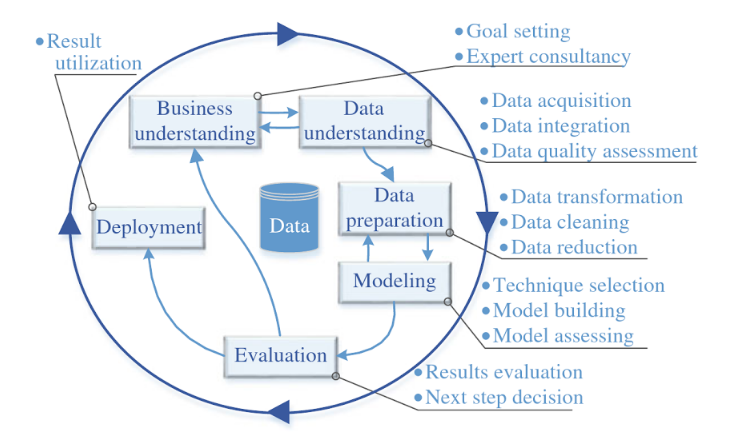
\includegraphics{CRISPDM.png}
\caption{Fluxo de processo do CRISP-DM}
\end{figure}

Como podemos observar na Figura 1, o fluxo de mineração de dados
seguindo a metodologia CRISP-DM é dividido em seis etapas, descritas
individualmente a seguir assim como elas foram aplicadas nesse projeto.

A. \emph{Entendimento do negócio}

É nessa etapa que o profissional que estará analisando os dados deve
procurar conhecer mais a respeito do ambiente no qual os dados foram
obtidos para entender melhor o real significado dos dados que serão
trabalhados.

Nesse projeto essa etapa consistiu em uma pesquisa a respeito dos cursos
de Direito, Ciência da Informação e Comunicação na universidade de
Brasília e a conversa com por e-mail com professores dos cursos.

B. \emph{Compreensão dos dados}

Nessa segunda etapa o objetivo é inspecionar, organizar e conhecer quais
dados temos a nossa disposição para análise.

A bases de dados que serão utilizadas nesse projeto são a OASIS, BDTD e
de publicações dos cursos mencionados acima.

C. \emph{Preparação dos dados}

Nessa etapa realizamos a limpeza dos dados para ser possível
trabalharmos com eles nas próximas etapas, seguindo o padrão de `tidy
data'.

D. \emph{Modelagem}

É nessa etapa que a mineração dos dados ocorre de fato, iniciamos com
uma análise preditiva das possíveis relações dos dados e com uma análise
mais profunda as predições iniciais podem ser validadas, além de termos
novos insights a respeito dos dados durante esse processo de validação.

E. \emph{Avaliação}

A avaliação é uma validação mais qualitativa que quantitativa, isto é,
uma validação se os resultados obtidos na modelagem são realmente úteis.
Essa etapa é essencial quando a análise dos dados está sendo feita para
um cliente, pois com ela os cientistas de dados podem ter uma ideia
melhor se os resultados das análises estão de acordo com o que o cliente
espera.

F. \emph{Desenvolvimento}

Agora com todas as validações e ultimos ajustes nos algoritmos de
análise dos dados, o modelo de mineração finalmente pode começar a ser
aplicado em soluções de problemas reais.

\subsection{Modelo de Referência
CRISP-DM}\label{modelo-de-referencia-crisp-dm}

Miner (2012), aprofunda: ``(\ldots{}) In CRISP-DM, the complete life
cycle of a data mining project is represented with \textbf{six phases}:
business understanding (determining the purpose of the study), data
understanding (data exploration and understanding), data preparation,
modeling, evaluation, and deployment.(\ldots{}). {[}Miner, Gary.
Practical Text Mining and Statistical Analysis for Non-structure Text
Data Applications. Academic Press, 2012.{]}

\subsubsection{Por que usar o CRISP-DM?}\label{por-que-usar-o-crisp-dm}

Imagine uma analogia entre um projeto de datamining e a preparação de
uma receita de bolo para ser usada em uma fábrica. Para iniciar a
produção, com base numa receita de comprovada eficácia (metodológica e
científica), você tem que minerar os ingredientes (dados) em um grande
supermercado (\emph{dataset}). Com os ingredientes você precisa aplicar
um método (a forma de misturá-los), colocar os ingredientes numa
determinada ordem, mexer por um certo tempo, aquecer por tantos minutos
até o bolo ficar pronto e ser aprovado em um ou mais testes de
degustação.

Tendo por objetivo fazer com que essa receita (script de mineração de
dados) possa ser executada com sucesso diversas vezes, numa fábrica,
será que outro cozinheiro (cientista) que reproduzisse a receita
(método) chegaria ao mesmo resultado? Se a metodologia (receita) já foi
bastante testada, então é bem provável que o resultado será o mesmo e
seu produto (receita de bolo) será aceito para a produção
(\emph{deployment}) de análises para consumo futuro, com base em
fundamentos científicos.

\subsubsection{Organização hierárquica de atividades em
fases}\label{organizacao-hierarquica-de-atividades-em-fases}

Dentro de cada fase no CRISP-DM existe uma estrutura hierárquica de
atividades genéricas para serem realizadas. Cada uma dessas atividades
\textbf{genéricas} pode determinar a execução de atividades
\textbf{específicas}.

Voltando ao exemplo do bolo, a atividade '' 1. Entendimento do Bolo''
poderia conter uma atividade genérica chamada ``1.1. Determinar para que
o bolo servirá (simples café da manhã? bolo de aniversário? bolo de
casamento?)``. Dentro dessa atividade genérica poderia haver atividades
específicas como ``1.1.1.Entrevistar o contratante para obter detalhes
de onde o bolo será usado?``; ``1.1.2. Conversar com os convidados sob
alguma necessidade especial (sem lactose? sem glútem?)``, etc.

\subsubsection{Seis Fases do CRISP-DM}\label{seis-fases-do-crisp-dm}

Com base no apresentado, segue uma descrição um pouco mais detalhada das
seis fases de um projeto no CRISP-DM, interpretadas no contexto do
relatório que você e seu grupo deverão produzir.

Todas as fases deverão ser adequadamente relatadas no relatório, em
seções que aparecem após a seçãoda metodologia

\begin{enumerate}
\def\labelenumi{\arabic{enumi}.}
\tightlist
\item
  O propósito da fase de \textbf{Entendimento do Negócio} é o
  desenvolvimento dos objetivos e declaração das necessidades do projeto
  sob a perspectiva do negócio, para transformar isso tudo em definição
  de um problema de data mining.
\end{enumerate}

As atividades genéricas dentro dessa fase envolvem:

\begin{itemize}
\item
  Identificar o que a organização realmente necessita alcançar. No caso
  específico desta disciplina, a necessidade do Sistema Nacional de
  Pós-Graduação do Brasil de produzir análises de alta qualidade de suas
  pós-graduações, com baixo custo. Como produzir um projeto de mineração
  de dados se você não sabe o que necessita encontrar ou resolver? Se
  você não entender os objetivos da organização pode levar ao erro de
  procurar as respostas certas para as perguntas erradas.
\item
  Avaliação das Circunstâncias. Envolve identificar quais recursos ou
  dificuldades podem influenciar os objetivos da mineração ou do projeto
  em si. No caso específico desta disciplina, isso envolve refletir,
  entre vários outros aspectos, sobre as limitações de tempo do projeto,
  que precisa ser realizado dentro de um semestre letivo, de modo que
  considerável parte das atividades já foram pré-organizadas pelos
  docentes responsáveis pela disciplina.
\item
  O projeto de mineração é o grande objetivo desta etapa e o relatório
  precisa conter uma seção sobre Metodologia, apresentando em detalhes o
  que se pretende fazer adiante.
\end{itemize}

\begin{enumerate}
\def\labelenumi{\arabic{enumi}.}
\setcounter{enumi}{1}
\tightlist
\item
  A fase de \textbf{Entendimento dos Dados} inicia determinando quais
  são os dados realmente disponíveis na organização, se existe permissão
  para utilizá-los, se existem dados confidenciais ou cobertos pelo
  sigilo. Por exemplo, um \emph{dataset} das declarações de imposto de
  renda da Receita Federal certamente seria protegido pelo sigilo
  fiscal. Dados de pacientes de hospitais podem conter restrições.
\end{enumerate}

Também é necessário acessar os dados para compreendê-los melhor para ter
o \emph{insight} de como será feita a modelagem mais tarde.

Na fase de entendimento dos dados pode-se trabalhar com quatro
atividades genéricas:

\begin{itemize}
\item
  Coleta inicial dos dados. Essa atividade envolve a análise das
  permissões de acesso e outras questões envolvendo sigilo e outros
  proprietários dos dados (terceiros). Por exemplo, eu poderia estar
  acessando uma base de dados que foi obtida de outro órgão por
  convênio, mas nesse convênio (contrato) não foi dada permissão para
  qualquer outro tipo de acesso ou exploração dos dados. Neste projeto,
  a coleta inicial foi feita pelos autores deste relatório. O relatório
  final deve conter indicações de como foi realizada a coleta inicial
  dos dados.
\item
  Descrição dos dados. A descrição dos dados verifica se os dados sendo
  acessados terão potencial para responder às questões de \emph{data
  mining}. Além disso, deve-se avaliar qual o volume de dados, a
  estrutura dos dados (tipos), codificações usadas, etc. Neste projeto,
  a descrição dos dados é responsabilidade parcial dos alunos, tendo em
  vista que este modelo já oferece uma descrição inicial. O relatório
  final deve conter descrições significativas e aprofundadas dos dados.
\item
  Análise exploratória dos dados. A análise exploratória dos dados
  possibilita um entendimento mais profundo da relação estatística
  existente entre os dados dos \emph{datasets} para um melhor
  entendimento da qualidade daqueles dados para o objetivo do projeto.
  Neste projeto, a análise exploratória dos dados é responsabilidade
  parcial dos alunos, tendo em vista que este relatório apresenta uma
  análise exploratória preliminar. O relatório final deve conter
  análises exploratórias dos dados que sejam significativas e
  aprofundadas.
\item
  Verificação da qualidade dos dados. A verificação da qualidade dos
  dados envolve responder se os dados disponíveis estão realmente
  completos. As informações disponíveis são suficientes para o trabalho
  proposto? Neste projeto, a verificação da qualidade dos dados é
  responsabilidade dos alunos.
\end{itemize}

\begin{enumerate}
\def\labelenumi{\arabic{enumi}.}
\setcounter{enumi}{2}
\tightlist
\item
  Na fase de \textbf{Preparação dos Dados} os \emph{datasets} que serão
  utilizados em todo o trabalho são construídos a partir dos dados
  brutos. Aqui os dados são ``filtrados'' retirando-se partes que não
  interessam e selecionando-se os ``campos'' necessários para o trabalho
  de mineração.
\end{enumerate}

São 5 as atividades genéricas nesta fase de preparação dos dados:

\begin{itemize}
\item
  Seleção dos dados. Envolve identificar quais dados, da nossa
  ``montanha de dados'', serão realmente utilizados. Quais variáveis dos
  dados brutos serão convertidas para o \emph{dataset}? Não é raro
  cometer o erro de selecionar dados para um modelo preditivo com base
  em uma falsa ideia de que aqueles dados contém a resposta para o
  modelo que se quer construir. Surge o cuidado de se separar o sinal do
  ruído (Silver, Nate. The Signal and the Noise: Why so many predictions
  fail --- but some don't. USA: The Penguin Press HC, 2012.).
\item
  Limpeza dos dados.
\item
  Construção dos dados. Envolve a criação de novas variáveis a partir de
  outras presentes nos \emph{datasets}.
\item
  Integração dos dados. Envolve a união (merge) de diferentes tabelas
  para criar um único \emph{dataset} para ser utilizado no R, por
  exemplo.
\item
  Formatação dos dados. Envolve a realização de pequenas alterações na
  estrutura dos dados, como a ordem das variáveis, para permitir a
  execução de determinado método de data mining.
\end{itemize}

\begin{enumerate}
\def\labelenumi{\arabic{enumi}.}
\setcounter{enumi}{3}
\tightlist
\item
  A fase de \textbf{Modelagem} no CRISP-DM envolve a construção e
  avaliação do modelo, podendo ser realizada em quatro atividades
  genéricas:
\end{enumerate}

\begin{itemize}
\item
  Seleção das técnicas de modelagem.
\item
  Realização de testes de modelagem, onde diferentes modelos são
  previamente testados e avaliados. Pode-se dividir o \emph{dataset}
  criado na etapa anterior para se ter uma base de treino na construção
  de modelos, e outra pequena parte para validar e avaliar a eficiência
  de cada modelo criado até se chegar ao mais ``eficiente''.
\item
  Construção do modelo definitivo, com base na melhor experiência do
  passo anterior.
\item
  Avaliação do modelo.
\end{itemize}

\begin{enumerate}
\def\labelenumi{\arabic{enumi}.}
\setcounter{enumi}{4}
\tightlist
\item
  Na fase de \textbf{Avaliação} do CRISP-DM os resultados não são apenas
  avaliados, mas se verifica se existem questões relacionadas à
  organização que não foram suficientemente abordadas. Deve-se refletir
  se o uso arepetido do modelo criado pode trazer algum ``efeito
  colateral'' para a organização.
\end{enumerate}

Nesta fase, pode-se trabalhar com 3 atividades genéricas:

\begin{itemize}
\item
  Avaliação dos resultados
\item
  Revisão do processo, por meio da qual verifica-se se o modelo foi
  construído adequadamente. As variáveis (passadas) para construir o
  modelo estarão disponíveis no futuro?
\item
  Determinação dos etapas seguintes. Pode ser necessário decidir-se por
  finalizar o projeto, passar à etapa de desenvolvimento, ou rever
  algumas fases anteriores para a melhoria do projeto.
\end{itemize}

\begin{enumerate}
\def\labelenumi{\arabic{enumi}.}
\setcounter{enumi}{5}
\tightlist
\item
  Na fase de \textbf{Implantação} (\emph{deployment}) se realiza o
  planejamento de implantação dos produtos desenvolvidos (scripts, no
  caso do executado nesta disciplina) para o ambiente operacional, para
  seu uso repetitivo, envolvendo atividades de monitoramento e
  manutenção do sistema (script) desenvolvido. A fase de implantação
  concluir com a produção e apresentação do relatório final com os
  resultados do projeto.
\end{enumerate}

São atividades genéricas na fase de \textbf{implantação}:

\begin{itemize}
\tightlist
\item
  Planejamento da transição dos produtos;
\item
  Planejamento do monitoramento dos produtos em utilização no ambiente
  operacional;
\item
  Planejamento de manuteção a ser eventualmente efetuada no produto
  (scripts);
\item
  Produção do relatório final;
\item
  Apresentação do relatório final;
\item
  Revisão sobre a execução do projeto, com registro de lições aprendidas
  etc.
\end{itemize}

No contexto do projeto realizado no âmbito desta disciplina, a
responsabilidade por execução de todas essas atividades é dos alunos,
com exceção da apresentação do relatório final, que não será realizada.

\section{CRISP-DM Fase 1 - Entendimento do
Negócio}\label{crisp-dm-fase-1---entendimento-do-negocio}

\subsection{O que é o Sistema Nacional de Pós-Graduação?
(Contextualização)}\label{o-que-e-o-sistema-nacional-de-pos-graduacao-contextualizacao}

A produção do conhecimento científico, no Brasil, é predominantemente
efetuada por meio do Sistema Nacional de Pós-Graduação - SNPG, e mais
fortemente relacionada com a formação de doutores nesse sistema (Pátaro
e Mezzomo, 2013), por meio de cursos de pós-graduação \emph{strictu
sensu}.

Fernandes e Sampaio (2017) já indicaram que a ciência é reconhecidamente
um elemento essencial para o desenvolvimento social e econômico de
qualquer nação. Assim sendo, faz-se mister aprimorar o SNPG como forma
de promoção desse crescimento, visando maximizar o retorno decorrente do
emprego dos recursos nele aplicados. A promoção do crescimento do SNPG
se dá predominantemente por meio de avaliações regulares de seus
programas de pós-graduação, sob responsabilidade da CAPES, que realiza a
cada quatro anos um complexo (Leite, 2018, p.~13) e custoso processo de
coleta de dados, análise e deliberação sobre as pós-graduações
\emph{strictu sensu}, em coerência com o estabelecido no Plano Nacional
de Pós-Graduação (PNPG) 2012-2020 (CAPES, 2010) e nos diversos
documentos que definem os critérios de organização da pós-graduação em
cada área do conhecimento (CAPES, 2018). Leite (2018) faz uma
apresentação geral de como se organizam e são avaliadas as
pós-graduações no Brasil.

O Plano Nacional de Pós-Graduação (PNPG), por outro lado, define
diretrizes estratégicas para desenvolvimento da pós-graduação
brasileira, que deve abordar prioritariamente grandes temas de interesse
nacional, tais como a redução das assimetrias de desenvolvimento entre
as regiões do Brasil, a formação de professores para a educação básica,
a formação de recursos humanos para as empresas, a resposta aos grandes
desafios brasileiros sobre Água, Energia, Transporte, Controle de
Fronteiras, Agronegócio, Amazônia, Amazônia Azul (Mar), Saúde, Defesa,
Programa Espacial, além de Justiça, Segurança Pública, Criminologia e
Desequilíbrio Regional. O PNPG também traça as diretrizes para
financiamento da pós-graduação e sua internacionalização, apresentando
conclusões e recomendações.

As avaliações do SNPG, ao atribuirem mensurações de desempenho às
diversas pós-graduações que dele fazem parte, geram incentivos e
penalidades aos programas, tendo em vista a limitada disponibilidade de
recursos para investimento em bolsas, taxas de bancada etc. Embora o
sistema seja altamente sofisticado ele é também altamente criticado
(Azevedo et al., 2016), sobretudo porque há percalços na busca por um
equilíbrio entre as diferentes concepções de finalidade da ciência. Se
de um lado a promoção do conhecimento gerado predominantemente nas ditas
ciências \emph{hard} constribui para criar fluxos econômicos mais
intensos, isso não significa que essa promoção possa ocorrer em
detrimento da menor promoção na geração de conhecimento sobre problemas
sociais, predominantemente gerado nas ditas ciências \emph{soft},
especialmente das áreas de humanidades, sob pena de ampliação de
desigualdades (Azevedo et al., 2016).

Não há solução simples, mas postula-se, nesta disciplina, que uma maior
agilidade na avaliação e a utilização de critérios mais objetivos,
poderá facilitar a melhoria do sistema.

\subsection{A UnB dentro do Sistema Nacional de Pós-Graduação
(Contextualização)}\label{a-unb-dentro-do-sistema-nacional-de-pos-graduacao-contextualizacao}

\subsubsection{O que é a UnB?}\label{o-que-e-a-unb}

A Universidade de Brasília (UnB) foi inaugurada, em 21 de abril de 1962,
após dois anos da criação de Brasília. A criação da Universidade foi
fruto do sonho e do trabalho de educadores como Darcy Ribeiro e Anísio
Teixeira.

As regras, a estrutura e concepção da Universidade foram definidas pelo
Plano Orientador, uma espécie de Carta Magna, datada de 1962, e ainda
hoje em vigor. O Plano foi a primeira publicação da Editora UnB e mostra
o espírito inovador da instituição. ``Só uma universidade nova,
inteiramente planificada, estruturada em bases mais flexíveis, poderá
abrir perspectivas de pronta renovação do nosso ensino superior'', diz o
Plano Orientador.

Hoje a Universidade de Brasília é formada por 4 campis, a Faculdade UnB
Planaltina (FUP), a primeira fora do Plano Piloto, a Faculdade de
Ceilândia (FCE) e a Faculdade do Gama (FGA) e o Campus Universitário
Darcy Ribeiro.

A missão da Universidade é ser uma instituição inovadora, comprometida
com a excelência acadêmica, científica e tecnológica formando cidadãos
conscientes do seu papel transformador na sociedade, respeitadas a ética
e a valorização de identidades e culturas com responsabilidade social.

\subsubsection{Descrição das pós-graduações da
UnB}\label{descricao-das-pos-graduacoes-da-unb}

O programa de pós-gradução da faculdade de comunicação (FAC) é divido em
dois grupos: mestrado e doutorado. Além disso, o Programa de
Pós-Graduação em Comunicação da Faculdade de Comunicação da Universidade
de Brasília (PPG/FAC/UnB) completou, em 2018, 44 anos de atividades
ininterruptas de formação e pesquisa de excelência na área. Com um
Mestrado consolidado, em atividade desde 1974, e um Doutorado de alto
padrão, instalado em 2003, o PPG/FAC/UnB, por sua localização central,
tem marcado sua atuação por uma forte inserção regional, nacional e
mesmo internacional e pela formação de novos quadros qualificados para o
ensino, a pesquisa e a extensão principalmente para as regiões
Centro-Oeste e Norte.

O Programa, a partir de suas quatro linhas de pesquisa, tem reconhecido
destaque nos estudos da Comunicação e da Sociedade, com ênfase em
epistemologia, teorias e tecnologias de comunicação, políticas de
comunicação e de cultura (das quais é pioneiro no Brasil), jornalismo
(com atualizado enfoque para as transformações estruturais) e estudos de
linguagens e narrativas. Os docentes são líderes de grupos de pesquisa e
têm se dedicado a um intenso esforço de publicação em conjunto com os
discentes do Programa e parceiros de pesquisa (o que pode ser atestado
pelos indicadores quantitativos e qualitativos da produção intelectual).

Ao longo dos 43 anos de atividade do Mestrado e 14 anos de existência do
Doutorado, o PPG/FAC/UnB formou 522 Mestres e 112 Doutores.

Já o curso de Direito da Universidade de Brasília foi criado junto com a
Universidade em 1962, dentro do Instituto Central de Ciências Humanas
(ICCH) até a criação da Faculdade de Ciências Jurídicas e Sociais
(FCJS), em 1967.

O curso de mestrado em Direito foi criado apenas em 1975. O curso de pós
graduação em direito na Universidade de Brasília possui um grande foco
em Direito e Estado, sendo referencia nacinal nos estudos de Direito
Público.

Atualmente o curso de graduação é oferecido tanto no período diurno como
noturno e os coordenadores dos cursos de cada período são,
respectivamente, Professor Henrique Araújo Costa e a Professora Inez
Lopes. O coordenador dos cursos de pós-graduação é o Professor Valcir
Gassen.

A Faculdade de Direito da Universidade de Brasília tembém possui um
periódico anual chamado Revista Direito.UnB no qual são publicados
artigos de alunos e professores.

E, por fim, o Programa de Pós--graduação em Ciência da Informação
(PPGCInf), da Faculdade de Ciência da Informação (FCI), da Universidade
de Brasília (UnB), visa aprofundar os conhecimentos adquiridos por
graduados e pós-graduados em cursos superiores, regulamentados pelos
órgãos competentes no Brasil, com interesses afins ao Programa,
dando-lhes oportunidade de desenvolver competência científica e
capacidade profissional e criadora em Ciência da Informação, formando
pesquisadores, professores e profissionais de alto nível, aptos a
desenvolver pesquisas e realizar inovações nesta área do saber. O
PPGCInf tem como área de concentração: Gestão da Informação. O PPGCInf
compreende os cursos de Mestrado Acadêmico e Doutorado (stricto sensu)
na área de Ciência da Informação.

O Mestrado Acadêmico objetiva promover a competência científica de
graduados, contribuindo para a formação de docentes e pesquisadores na
área da informação. O Doutorado visa formar profissionais de alto nível,
que possam atuar como pesquisadores autônomos e como docentes na área de
Ciência da Informação, buscando: propiciar visão abrangente da área;
desenvolver sólida base teórica relativa à área; estimular o
desenvolvimento da produção científica da área, com projetos de pesquisa
inovadores e socialmente relevantes.

A Linha de Pesquisa Organização da Informação busca propor conhecimentos
nos níveis epistemológico, científico e prático relativos à origem,
coleta, organização, estocagem, recuperação, interpretação, transmissão,
transformação e uso da informação. Neste contexto, relaciona-se com a
natureza da informação, a terminologia e modelos de tratamento e
recuperação de informações; as necessidades dos usuários de informação e
suas implicações; a identificação dos recursos necessários a partir dos
tipos e formatos; a identificação, o tratamento e a recuperação de
informações adequadas para o usuário; a formulação de políticas,
estratégias, planejamentos, normas e processos relacionados a diferentes
espaços de informação.

A Linha de Pesquisa Comunicação e Mediação da Informação reúne estudos
que buscam conhecimentos nos níveis epistemológico, científico e prático
sobre processos de comunicação em diversos contextos e setores da
sociedade. Os estudos desenvolvidos sob esta linha privilegiam a busca
pelo entendimento dos fenômenos relacionados ao fluxo da informação, os
atores que deles participam e os canais utilizados. Os estudos dessa
linha contemplam ainda fatores internos e externos que influenciam tais
fluxos e a produção e aplicação de indicadores para sua avaliação. A
linha inclui também estudos sobre políticas, estratégias e planejamento
dos processos de comunicação nos diversos contextos e setores da
sociedade e desdobramentos sociais, políticos, culturais e econômicos da
comunicação e acesso à informação, e ainda estudos relacionados às
profissões ligadas a esses processos.

\subsubsection{Outros aspectos que caracterizam a produção científica e
acadêmica da
UnB}\label{outros-aspectos-que-caracterizam-a-producao-cientifica-e-academica-da-unb}

Texto a desenvolver.

\subsection{O que a Organização precisa realmente
alcançar?}\label{o-que-a-organizacao-precisa-realmente-alcancar}

Vários stakeholders estão envolvidos no projeto em curso, e poderíamos
considerar cada um deles como distintas organizações que possuem
interesses distintos e complementares. Elas são: * A Disciplina Ciência
de Dados para Todos 2018.1, que quer comprovar que seus alunos dominam
ferramentas e técnicas de ciência de dados, para fins de avaliação de
rendimento da disciplina. * A UnB, representada pelos decanatos de
pós-graduação (DPG) e de pesquisa e inovação (DPI), que querem dispor de
instrumentos para realização de avaliações contínuas de suas
pós-graduações. * O SNPG, que assim com o DPG e DPI, também pode se
beneficiar do uso de instrumentos para realização de avaliações
contínuas de suas pós-graduações. * Os interessados em melhor conhecer o
que é produzido pelo Sistema Nacional de Pós-graduação, como empresas
privadas, que querem desfrutar dos benefícios gerados pela ciência
brasileira.

A fim de dar maior fidelidade e homogeneidade ao exercício realizado na
disciplina, focaremos em atendimento aos interesses comuns das
organizações DPI, DPG e CAPES, que desejam dispor de instrumentos ágeis
para avaliação contínua da pós-graduação brasileira.

Com base no exposto, o objetivo do trabalho final a ser alcançado pelos
produtos d emineração de dados desenvolvido pelos alunos da disciplina
Ciência de Dados para Todos é produzir, tomando por base inicial os
dados fornecidos pelos professores responsáveis pela disciplina,
ferramentas para análise e avaliação contínuas e de baixo custo, do
desempenho de um conjunto de pós-graduações que estão vinculadas a uma
mesma subárea ou grupo de conhecimento. Cada área de pós-graduação
apresenta suas características peculiares, assim como cada um dos
programas vinculados a essas áreas. Como já informado, características
peculiares de cada programa podem ser obtidas a partir de visita ao
sítio da CAPES (2018).

\subsection{Avaliação das
Circunstâncias}\label{avaliacao-das-circunstancias}

Este documento serve como base para a realização dos trabalhos dos
alunos. apresenta limitações no tocante à quantidade pequena de dados
que serão empregados para análises e avaliações, tendo em vista sua
finalidade maior que é a didática, de permitir aos alunos demonstrarem a
capacidade de aplicação das técnicas e ferramentas apreendidas durante o
semestre.

\subsubsection{Avaliação preliminar das pós-graduações na
UnB}\label{avaliacao-preliminar-das-pos-graduacoes-na-unb}

Texto a desenvolver.

\subsubsection{Avaliação preliminar da produção científica e acadêmica
da
UnB}\label{avaliacao-preliminar-da-producao-cientifica-e-academica-da-unb}

Texto a desenvolver.

\section{CRISP-DM Fase 2 - Entendimento dos
Dados}\label{crisp-dm-fase-2---entendimento-dos-dados}

Doravante, a fim de facilitar aos alunos seguirem a metodologia
CRISP-DM, os nomes das seções e subseções de texto serão prefixadas com
o número e nome da fase e atividade genérica do CRISP-DM. Fica facultado
aos grupos seguir ou não a sequência prevista, tendo em vista que se
pode retornar às fases anteriores, bem como podem haver atividades que
não foram adequadas às características do problema específico sob
análise.

\subsection{CRISP-DM Fase.Atividade 2.1 - Coleta inicial dos
dados}\label{crisp-dm-fase.atividade-2.1---coleta-inicial-dos-dados}

Todos os arquivos com dados iniciais a seguir apresentados foram
fornecidos pelos professores responsáveis pela disciplina. Os dados
foram gerados no mês de maio de 2018, e compilam informações entre os
anos de 2010 e 2017. Os arquivos estão no formato JSON, e seus atributos
iniciais e conteúdos são apresentados a seguir.

\subsubsection{Perfil profissional dos docentes vinculados às
pós-graduações do curso de direito, comunicação e ciência da
informação}\label{perfil-profissional-dos-docentes-vinculados-as-pos-graduacoes-do-curso-de-direito-comunicacao-e-ciencia-da-informacao}

\begin{Shaded}
\begin{Highlighting}[]
\NormalTok{json.perfil_ci <-}\StringTok{ "data/CI.profile.json"}
\KeywordTok{file.info}\NormalTok{(json.perfil_ci)}
\end{Highlighting}
\end{Shaded}

\begin{verbatim}
##                         size isdir mode               mtime
## data/CI.profile.json 1126228 FALSE  666 2018-07-07 19:37:00
##                                    ctime               atime exe
## data/CI.profile.json 2018-07-07 19:37:00 2018-07-07 19:37:00  no
\end{verbatim}

\begin{Shaded}
\begin{Highlighting}[]
\NormalTok{json.perfil_comunicacao <-}\StringTok{ "data/Comunicacao.profile.json"}
\KeywordTok{file.info}\NormalTok{(json.perfil_comunicacao)}
\end{Highlighting}
\end{Shaded}

\begin{verbatim}
##                                  size isdir mode               mtime
## data/Comunicacao.profile.json 1247316 FALSE  666 2018-07-07 19:37:00
##                                             ctime               atime exe
## data/Comunicacao.profile.json 2018-07-07 19:37:00 2018-07-07 19:37:00  no
\end{verbatim}

\begin{Shaded}
\begin{Highlighting}[]
\NormalTok{json.perfil_direito <-}\StringTok{ "data/Direito.profile.json"}
\KeywordTok{file.info}\NormalTok{(json.perfil_direito)}
\end{Highlighting}
\end{Shaded}

\begin{verbatim}
##                              size isdir mode               mtime
## data/Direito.profile.json 1782980 FALSE  666 2018-07-07 19:37:01
##                                         ctime               atime exe
## data/Direito.profile.json 2018-07-07 19:37:01 2018-07-07 19:37:01  no
\end{verbatim}

Os arquivos ``CI.profile.json'', ``Comunicacao.profile.json'' e
``Direito.profile.json'' apresentam dados sobre o perfil de todos os
docentes vinculados a programas de pós-graduação da UnB, entre 2010 e
2017, nos cursos citados anteriormente.

Esse arquivo foi fornecido pelos docentes responsáveis pela disciplina.

\subsubsection{Orientações de mestrado e doutorado realizadas pelos
docentes vinculados às
pós-graduações}\label{orientacoes-de-mestrado-e-doutorado-realizadas-pelos-docentes-vinculados-as-pos-graduacoes}

\begin{Shaded}
\begin{Highlighting}[]
\NormalTok{json.advise_ci <-}\StringTok{ "data/CI.advise.json"}
\KeywordTok{file.info}\NormalTok{(json.advise_ci)}
\end{Highlighting}
\end{Shaded}

\begin{verbatim}
##                       size isdir mode               mtime
## data/CI.advise.json 526741 FALSE  666 2018-07-07 19:37:00
##                                   ctime               atime exe
## data/CI.advise.json 2018-07-07 19:37:00 2018-07-07 19:37:00  no
\end{verbatim}

\begin{Shaded}
\begin{Highlighting}[]
\NormalTok{json.advise_comunicacao <-}\StringTok{ "data/Comunicacao.advise.json"}
\KeywordTok{file.info}\NormalTok{(json.advise_comunicacao)}
\end{Highlighting}
\end{Shaded}

\begin{verbatim}
##                                size isdir mode               mtime
## data/Comunicacao.advise.json 569439 FALSE  666 2018-07-07 19:37:00
##                                            ctime               atime exe
## data/Comunicacao.advise.json 2018-07-07 19:37:00 2018-07-07 19:37:00  no
\end{verbatim}

\begin{Shaded}
\begin{Highlighting}[]
\NormalTok{json.advise_direito <-}\StringTok{ "data/Direito.advise.json"}
\KeywordTok{file.info}\NormalTok{(json.advise_direito)}
\end{Highlighting}
\end{Shaded}

\begin{verbatim}
##                            size isdir mode               mtime
## data/Direito.advise.json 934056 FALSE  666 2018-07-07 19:37:00
##                                        ctime               atime exe
## data/Direito.advise.json 2018-07-07 19:37:00 2018-07-07 19:37:00  no
\end{verbatim}

Os arquivos ``CI.advise.json'', ``Comunicacao.advise.json'' e
``Direito.advise.json'' apresentam dados sobre o orientações de mestrado
e doutorado feitas por todos os docentes vinculados a programas de
pós-graduação da UnB, entre 2010 e 2017, dos cursos citados na seção
anterior.

Esse arquivo foi fornecido pelos docentes responsáveis pela disciplina.

\subsubsection{Produção bibliográfica gerada pelos docentes vinculados
às
pós-graduações}\label{producao-bibliografica-gerada-pelos-docentes-vinculados-as-pos-graduacoes}

\begin{Shaded}
\begin{Highlighting}[]
\NormalTok{json.producao.bibliografica_ci <-}\StringTok{ "data/CI.publication.json"}
\KeywordTok{file.info}\NormalTok{(json.producao.bibliografica_ci) }
\end{Highlighting}
\end{Shaded}

\begin{verbatim}
##                            size isdir mode               mtime
## data/CI.publication.json 465994 FALSE  666 2018-07-07 19:37:00
##                                        ctime               atime exe
## data/CI.publication.json 2018-07-07 19:37:00 2018-07-07 19:37:00  no
\end{verbatim}

\begin{Shaded}
\begin{Highlighting}[]
\NormalTok{json.producao.bibliografica_comunicacao <-}\StringTok{ "data/Comunicacao.publication.json"}
\KeywordTok{file.info}\NormalTok{(json.producao.bibliografica_comunicacao) }
\end{Highlighting}
\end{Shaded}

\begin{verbatim}
##                                     size isdir mode               mtime
## data/Comunicacao.publication.json 539523 FALSE  666 2018-07-07 19:37:00
##                                                 ctime               atime
## data/Comunicacao.publication.json 2018-07-07 19:37:00 2018-07-07 19:37:00
##                                   exe
## data/Comunicacao.publication.json  no
\end{verbatim}

\begin{Shaded}
\begin{Highlighting}[]
\NormalTok{json.producao.bibliografica_direito <-}\StringTok{ "data/Direito.publication.json"}
\KeywordTok{file.info}\NormalTok{(json.producao.bibliografica_direito) }
\end{Highlighting}
\end{Shaded}

\begin{verbatim}
##                                 size isdir mode               mtime
## data/Direito.publication.json 675135 FALSE  666 2018-07-07 19:37:01
##                                             ctime               atime exe
## data/Direito.publication.json 2018-07-07 19:37:01 2018-07-07 19:37:01  no
\end{verbatim}

Os arquivos ``CI.advise.json'', ``Comunicacao.advise.json'' e
``Direito.advise.json'' apresentam dados sobre a produção bibliográfica
gerada por todos os docentes vinculados a programas de pós-graduação da
UnB, entre 2010 e 2017, dos cursos citados na seção anterior.

\subsection{CRISP-DM Fase.Atividade 2.2 - Descrição dos
Dados}\label{crisp-dm-fase.atividade-2.2---descricao-dos-dados}

Como já informado, a descrição dos dados verifica se os dados sendo
acessados terão potencial para responder às questões de \emph{data
mining}. Além disso, deve-se avaliar qual o volume de dados, a estrutura
dos dados (tipos), codificações usadas, etc. Neste projeto, a descrição
dos dados é responsabilidade parcial dos alunos, tendo em vista que esta
seção já oferece uma descrição inicial simplificada. O relatório final
deve conter descrições significativas e aprofundadas dos dados.

\subsubsection{Descrição dos dados do
perfil}\label{descricao-dos-dados-do-perfil}

OS arquivoS ``CI.profile.json'',``Comunicacao.profile.json'' e
``Direito.profile.json'' que contém dados que caracterizam o perfil
profissional de todos os docentes do grupo, dos 3 cursos, sob análise,
podem ser lido por meio do comando seguinte.

\begin{Shaded}
\begin{Highlighting}[]
\NormalTok{unb.prof_ci <-}\StringTok{ }\KeywordTok{fromJSON}\NormalTok{(}\StringTok{"data/CI.profile.json"}\NormalTok{)}
\NormalTok{unb.prof_comunicacao <-}\StringTok{ }\KeywordTok{fromJSON}\NormalTok{(}\StringTok{"data/Comunicacao.profile.json"}\NormalTok{)}
\NormalTok{unb.prof_direito <-}\StringTok{ }\KeywordTok{fromJSON}\NormalTok{(}\StringTok{"data/Direito.profile.json"}\NormalTok{)}
\end{Highlighting}
\end{Shaded}

A quantidade de docentes de cada curso, sob análise, é apresentada a
seguir.

\begin{Shaded}
\begin{Highlighting}[]
\KeywordTok{length}\NormalTok{(unb.prof_ci)}
\end{Highlighting}
\end{Shaded}

\begin{verbatim}
## [1] 27
\end{verbatim}

\begin{Shaded}
\begin{Highlighting}[]
\KeywordTok{length}\NormalTok{(unb.prof_comunicacao)}
\end{Highlighting}
\end{Shaded}

\begin{verbatim}
## [1] 31
\end{verbatim}

\begin{Shaded}
\begin{Highlighting}[]
\KeywordTok{length}\NormalTok{(unb.prof_direito)}
\end{Highlighting}
\end{Shaded}

\begin{verbatim}
## [1] 37
\end{verbatim}

Para gerar uma apresentação inicial dos dados que estão contido nos
dados de perfil dos docentes de cada curso, pode-se usar a função
glimpse, da biblioteca dplyr, como ilustra o código seguinte, que
apresenta os atributos típicos que podem ser obtidos relativamente a um
pesquisador específico, o mais antigo docente ainda em exercício na UnB
a ter criado seu registro na plataforma Lattes.

\begin{Shaded}
\begin{Highlighting}[]
\KeywordTok{library}\NormalTok{(dplyr) }
\KeywordTok{glimpse}\NormalTok{(unb.prof_ci[[}\DecValTok{1}\NormalTok{]], }\DataTypeTok{width =} \DecValTok{30}\NormalTok{)}
\end{Highlighting}
\end{Shaded}

\begin{verbatim}
## List of 7
##  $ nome                  : chr "Fernando César Lima Leite"
##  $ resumo_cv             : chr "Graduado em Biblioteconomia. Mestre em Ciência da Informação. Doutor em Ciência da Informação. Experiência na á"| __truncated__
##  $ areas_de_atuacao      :'data.frame':  4 obs. of  4 variables:
##   ..$ grande_area  : chr [1:4] "CIENCIAS_SOCIAIS_APLICADAS" "CIENCIAS_SOCIAIS_APLICADAS" "CIENCIAS_SOCIAIS_APLICADAS" "CIENCIAS_SOCIAIS_APLICADAS"
##   ..$ area         : chr [1:4] "Ciência da Informação" "Ciência da Informação" "Ciência da Informação" "Ciência da Informação"
##   ..$ sub_area     : chr [1:4] "" "Comunicação Científica" "Biblioteconomia" "Gestão do Conhecimento"
##   ..$ especialidade: chr [1:4] "" "" "" "Gestão da informação e do conhecimento"
##  $ endereco_profissional :List of 8
##   ..$ instituicao: chr "Universidade de Brasília"
##   ..$ orgao      : chr "Faculdade de Ciência da Informação"
##   ..$ unidade    : chr ""
##   ..$ DDD        : chr "61"
##   ..$ telefone   : chr "33072641"
##   ..$ bairro     : chr "Asa Norte"
##   ..$ cep        : chr "70919900"
##   ..$ cidade     : chr "Brasília"
##  $ producao_bibiografica :List of 5
##   ..$ CAPITULO_DE_LIVRO                     :'data.frame':   3 obs. of  13 variables:
##   .. ..$ tipo                    : chr [1:3] "Capítulo de livro publicado" "Capítulo de livro publicado" "Capítulo de livro publicado"
##   .. ..$ titulo_do_capitulo      : chr [1:3] "Insumos conceituais e práticos para iniciativas de repositórios institucionais de acesso aberto à informação ci"| __truncated__ "Acesso Aberto no Brasil: aspetos históricos, ações institucionais e panorama atual" "Gestão integrada da informação científica e tecnológica e o acesso aberto: onde estamos e onde podemos chegar"
##   .. ..$ titulo_do_livro         : chr [1:3] "Implantação e gestão de repositórios institucionais: políticas, memória, livre acesso e preservação" "Uma década de acesso aberto na UMinho e no mundo" "Repositórios digitais: teoria e prática"
##   .. ..$ ano                     : chr [1:3] "2010" "2013" "2017"
##   .. ..$ doi                     : chr [1:3] "" "" ""
##   .. ..$ pais_de_publicacao      : chr [1:3] "Brasil" "Brasil" "Brasil"
##   .. ..$ isbn                    : chr [1:3] "9788523206550" "9789899870406" "9788570141972"
##   .. ..$ nome_da_editora         : chr [1:3] "EdUFBA" "Universidade do Minho, Serviços de Documentação" "EDUTFPR"
##   .. ..$ numero_da_edicao_revisao: chr [1:3] "" "1" "1"
##   .. ..$ organizadores           : chr [1:3] "MARCONDES, C. H.; SAYÃO, L. F.; TOUTAIN, L. B.; ROSA, F. G." "Eloy Rodrigues; Alma Swan; Ana Alice Baptista" "Vechiato, Fernando Luiz et al"
##   .. ..$ paginas                 : chr [1:3] "163 - 202" "133 - 150" "35 - 65"
##   .. ..$ autores                 :List of 3
##   .. ..$ autores-endogeno        :List of 3
##   ..$ DEMAIS_TIPOS_DE_PRODUCAO_BIBLIOGRAFICA:'data.frame':   1 obs. of  9 variables:
##   .. ..$ natureza          : chr "Cartilha"
##   .. ..$ titulo            : chr "Boas práticas para a construção de repositórios institucionais da produção científica"
##   .. ..$ ano               : chr "2012"
##   .. ..$ pais_de_publicacao: chr "Brasil"
##   .. ..$ editora           : chr "IBICT"
##   .. ..$ doi               : chr ""
##   .. ..$ numero_de_paginas : chr "34"
##   .. ..$ autores           :List of 1
##   .. ..$ autores-endogeno  :List of 1
##   ..$ EVENTO                                :'data.frame':   5 obs. of  11 variables:
##   .. ..$ natureza        : chr [1:5] "COMPLETO" "COMPLETO" "RESUMO" "RESUMO" ...
##   .. ..$ titulo          : chr [1:5] "Software livre para implementação de repositórios digitais e provedores de serviços: experiência da Embrapa Inf"| __truncated__ "Práticas de busca, acesso e disseminação da informação científica de pesquisadores de diferentes áreas do conhecimento" "Open Access publishing and academics? career assessment. Peer reviewers knowledge and opinions regarding open a"| __truncated__ "Políticas de acesso aberto das agências brasileiras de fomento à pesquisa" ...
##   .. ..$ nome_do_evento  : chr [1:5] "Jornadas Argentinas de Informática (Jornadas de Software Libre)" "Encontro Nacional de Pesquisa em Ciência da Informação -I ENANCIB" "Fourth International PKP Scholarly Publishing Conference" "4ª Conferência Luso-Brasileira sobre Acesso Aberto" ...
##   .. ..$ ano_do_trabalho : chr [1:5] "2010" "2012" "2013" "2013" ...
##   .. ..$ pais_do_evento  : chr [1:5] "Brasil" "Brasil" "Brasil" "Brasil" ...
##   .. ..$ cidade_do_evento: chr [1:5] "Caba, Argentina" "Rio de Janeiro" "Mexico City" "São Paulo" ...
##   .. ..$ doi             : chr [1:5] "" "" "" "" ...
##   .. ..$ classificacao   : chr [1:5] "NACIONAL" "NACIONAL" "INTERNACIONAL" "INTERNACIONAL" ...
##   .. ..$ paginas         : chr [1:5] "1 - 9" " - " " - " " - " ...
##   .. ..$ autores         :List of 5
##   .. ..$ autores-endogeno:List of 5
##   ..$ LIVRO                                 :'data.frame':   1 obs. of  13 variables:
##   .. ..$ titulo                  : chr "Repositórios institucionais da América Latina e o acesso aberto à informação científica"
##   .. ..$ ano                     : chr "2017"
##   .. ..$ tipo                    : chr "LIVRO_PUBLICADO"
##   .. ..$ natureza                : chr "TEXTO_INTEGRAL"
##   .. ..$ pais_de_publicacao      : chr "Brasil"
##   .. ..$ isbn                    : chr "9788570131201"
##   .. ..$ doi                     : chr ""
##   .. ..$ nome_da_editora         : chr "IBICT"
##   .. ..$ numero_da_edicao_revisao: chr "1"
##   .. ..$ numero_de_paginas       : chr ""
##   .. ..$ numero_de_volumes       : chr ""
##   .. ..$ autores                 :List of 1
##   .. ..$ autores-endogeno        :List of 1
##   ..$ PERIODICO                             :'data.frame':   13 obs. of  10 variables:
##   .. ..$ natureza        : chr [1:13] "COMPLETO" "COMPLETO" "COMPLETO" "COMPLETO" ...
##   .. ..$ titulo          : chr [1:13] "An Open Access Approach to Scientific Information Management at the Brazilian Agricultural Research Corporation" "Acesso aberto como estratégia de disseminação e preservação da produção científica discente: a Biblioteca Digit"| __truncated__ "Acesso aberto à informação científica em agricultura: a experiência da Empresa Brasileira de Pesquisa Agropecuá"| __truncated__ "Search, access and dissemination of scientific information from scientists, social scientists and humanists" ...
##   .. ..$ periodico       : chr [1:13] "Scholarly and Research Communication" "Bibliotecas Universitárias : pesquisas, experiências e perspectivas" "Liinc em Revista" "Biblios (Lima)" ...
##   .. ..$ ano             : chr [1:13] "2010" "2011" "2012" "2015" ...
##   .. ..$ volume          : chr [1:13] "1" "1" "8" "" ...
##   .. ..$ issn            : chr [1:13] "03163849" "21799504" "18083536" "15624730" ...
##   .. ..$ paginas         : chr [1:13] "1 - 12" "71 - 80" "414 - 430" "22 - 42" ...
##   .. ..$ doi             : chr [1:13] "" "" "10.18225/liinc.v8i2.503" "10.5195/biblios.2014.195" ...
##   .. ..$ autores         :List of 13
##   .. ..$ autores-endogeno:List of 13
##  $ orientacoes_academicas:List of 4
##   ..$ ORIENTACAO_CONCLUIDA_DOUTORADO  :'data.frame': 3 obs. of  13 variables:
##   .. ..$ natureza                   : chr [1:3] "Tese de doutorado" "Tese de doutorado" "Tese de doutorado"
##   .. ..$ titulo                     : chr [1:3] "Depósito da produção científica em repositórios institucionais de acesso aberto à informação científica" "Framework de interação humano-computador para o desenvolvimento de sistemas orientados à redução de assimetrias"| __truncated__ "Fatores que influenciam a comunicação de dados de pesquisa sobre o vírus da zika, na perspectiva de pesquisadores"
##   .. ..$ ano                        : chr [1:3] "2015" "2016" "2017"
##   .. ..$ id_lattes_aluno            : chr [1:3] "8636654005487585" "8743793460674396" "5676915146365703"
##   .. ..$ nome_aluno                 : chr [1:3] "Marília Augusta de Freitas" "José Antônio Machado do Nascimento" "Michelli Pereira da Costa"
##   .. ..$ instituicao                : chr [1:3] "Universidade de Brasília" "Universidade de Brasília" "Universidade de Brasília"
##   .. ..$ curso                      : chr [1:3] "Ciência da Informação" "Ciências da Informação" "Ciência da Informação"
##   .. ..$ codigo_do_curso            : chr [1:3] "90000011" "90000010" "90000005"
##   .. ..$ bolsa                      : chr [1:3] "NAO" "NAO" "SIM"
##   .. ..$ agencia_financiadora       : chr [1:3] "" "" "Conselho Nacional de Desenvolvimento Científico e Tecnológico"
##   .. ..$ codigo_agencia_financiadora: chr [1:3] "" "" "002200000000"
##   .. ..$ nome_orientadores          :List of 3
##   .. ..$ id_lattes_orientadores     :List of 3
##   ..$ ORIENTACAO_CONCLUIDA_MESTRADO   :'data.frame': 7 obs. of  13 variables:
##   .. ..$ natureza                   : chr [1:7] "Dissertação de mestrado" "Dissertação de mestrado" "Dissertação de mestrado" "Dissertação de mestrado" ...
##   .. ..$ titulo                     : chr [1:7] "Acesso aberto à informação científica: estudo sobre iniciativas desenvolvidas na Universidade Federal de Minas Gerais" "Gestão de teses e dissertações eletrônicas no contexto do acesso aberto à informação científica no Brasil" "Características e contribuições da via verde para o acesso aberto na América Latina" "Modelos de negócios de periodicos científicos da América Latina e Caribe" ...
##   .. ..$ ano                        : chr [1:7] "2010" "2013" "2014" "2014" ...
##   .. ..$ id_lattes_aluno            : chr [1:7] "" "8018556894529318" "5676915146365703" "1937356712603636" ...
##   .. ..$ nome_aluno                 : chr [1:7] "Raisa Mendes Fernandes de Souza" "Tainá Batista de Assis" "Michelli Pereira Costa" "Julio Francisco Santillan Aldana" ...
##   .. ..$ instituicao                : chr [1:7] "Universidade Federal de Minas Gerais" "Universidade de Brasília" "Universidade de Brasília" "Universidade de Brasília" ...
##   .. ..$ curso                      : chr [1:7] "Ciências da Informação" "Ciências da Informação" "Ciência da Informação" "Ciências da Informação" ...
##   .. ..$ codigo_do_curso            : chr [1:7] "32000286" "51500183" "90000002" "51500183" ...
##   .. ..$ bolsa                      : chr [1:7] "NAO" "NAO" "NAO" "SIM" ...
##   .. ..$ agencia_financiadora       : chr [1:7] "" "" "" "Conselho Nacional de Desenvolvimento Científico e Tecnológico" ...
##   .. ..$ codigo_agencia_financiadora: chr [1:7] "" "" "" "002200000000" ...
##   .. ..$ nome_orientadores          :List of 7
##   .. ..$ id_lattes_orientadores     :List of 7
##   ..$ ORIENTACAO_EM_ANDAMENTO_MESTRADO:'data.frame': 2 obs. of  13 variables:
##   .. ..$ natureza                   : chr [1:2] "Dissertação de mestrado" "Dissertação de mestrado"
##   .. ..$ titulo                     : chr [1:2] "Diretrizes internacionais para bibliotecas prisionais" "Periódicos científicos eletrônicos no contexto das publicações ampliadas"
##   .. ..$ ano                        : chr [1:2] "2016" "2016"
##   .. ..$ id_lattes_aluno            : chr [1:2] "2403536925847453" "1563407482755076"
##   .. ..$ nome_aluno                 : chr [1:2] "Luanna Vieira Leite" "Danyelle Mayara da Silva"
##   .. ..$ instituicao                : chr [1:2] "Universidade de Brasília" "Universidade de Brasília"
##   .. ..$ curso                      : chr [1:2] "Ciência da Informação" "Ciência da Informação"
##   .. ..$ codigo_do_curso            : chr [1:2] "90000012" "90000012"
##   .. ..$ bolsa                      : chr [1:2] "NAO" "NAO"
##   .. ..$ agencia_financiadora       : chr [1:2] "" ""
##   .. ..$ codigo_agencia_financiadora: chr [1:2] "" ""
##   .. ..$ nome_orientadores          :List of 2
##   .. ..$ id_lattes_orientadores     :List of 2
##   ..$ OUTRAS_ORIENTACOES_CONCLUIDAS   :'data.frame': 19 obs. of  13 variables:
##   .. ..$ natureza                   : chr [1:19] "TRABALHO_DE_CONCLUSAO_DE_CURSO_GRADUACAO" "TRABALHO_DE_CONCLUSAO_DE_CURSO_GRADUACAO" "TRABALHO_DE_CONCLUSAO_DE_CURSO_GRADUACAO" "TRABALHO_DE_CONCLUSAO_DE_CURSO_GRADUACAO" ...
##   .. ..$ titulo                     : chr [1:19] "Acesso aberto à informação científica: análise bibliométrica preliminar da literatura brasileira" "Modelo de gestão de repositórios institucionais de acesso aberto à informação científica" "Mapeamento e caracterização dos repositórios institucionais de acesso aberto à informação científica das univer"| __truncated__ "Estado atual das bibliotecas digitais das universidades federais do Brasil" ...
##   .. ..$ ano                        : chr [1:19] "2010" "2010" "2010" "2011" ...
##   .. ..$ id_lattes_aluno            : chr [1:19] "" "" "" "" ...
##   .. ..$ nome_aluno                 : chr [1:19] "Sílvia Regina Batista Mendonça" "Michelli Costa" "Janaina dos Santos Melo e Maria Fernanda Mascarenhas Melis" "Fabrícia da Silva Costa Feitosa e Ludmilla de Melo Silva" ...
##   .. ..$ instituicao                : chr [1:19] "Universidade de Brasília" "Universidade de Brasília" "Universidade de Brasília" "Universidade de Brasília" ...
##   .. ..$ curso                      : chr [1:19] "Biblioteconomia" "Biblioteconomia" "Biblioteconomia" "Biblioteconomia" ...
##   .. ..$ codigo_do_curso            : chr [1:19] "90000000" "90000000" "90000000" "90000000" ...
##   .. ..$ bolsa                      : chr [1:19] "NAO" "NAO" "NAO" "NAO" ...
##   .. ..$ agencia_financiadora       : chr [1:19] "" "" "" "" ...
##   .. ..$ codigo_agencia_financiadora: chr [1:19] "" "" "" "" ...
##   .. ..$ nome_orientadores          :List of 19
##   .. ..$ id_lattes_orientadores     :List of 19
##  $ senioridade           : chr "9"
\end{verbatim}

Uma breve inspeção visual dos atributos do curso de ciência da
informação anteriormente apresentados permite inferir que o pesquisador
sob análise:

\begin{itemize}
\tightlist
\item
  Atua predominantemente nas áreas de arquivologia, museologia e
  biblioteoconomia.
\item
  Trabalha no Instituto de Ciência de Informação da UnB.
\end{itemize}

\begin{Shaded}
\begin{Highlighting}[]
\KeywordTok{glimpse}\NormalTok{(unb.prof_comunicacao[[}\DecValTok{1}\NormalTok{]], }\DataTypeTok{width =} \DecValTok{30}\NormalTok{)}
\end{Highlighting}
\end{Shaded}

\begin{verbatim}
## List of 7
##  $ nome                  : chr "Dione Oliveira Moura"
##  $ resumo_cv             : chr "Professora e pesquisadora em Comunicação. Possui graduação em Comunicação Social - Jornalismo pela Universidade"| __truncated__
##  $ areas_de_atuacao      :'data.frame':  3 obs. of  4 variables:
##   ..$ grande_area  : chr [1:3] "CIENCIAS_SOCIAIS_APLICADAS" "CIENCIAS_SOCIAIS_APLICADAS" "CIENCIAS_SOCIAIS_APLICADAS"
##   ..$ area         : chr [1:3] "Comunicação" "Comunicação" "Ciência da Informação"
##   ..$ sub_area     : chr [1:3] "jornalismo científico e ambiental" "Jornalismo e Sociedade" "comunicação científica"
##   ..$ especialidade: chr [1:3] "" "" ""
##  $ endereco_profissional :List of 8
##   ..$ instituicao: chr "Universidade de Brasília"
##   ..$ orgao      : chr "Faculdade de Comunicação"
##   ..$ unidade    : chr ""
##   ..$ DDD        : chr "61"
##   ..$ telefone   : chr "33072295"
##   ..$ bairro     : chr "Asa Norte"
##   ..$ cep        : chr "70900-000"
##   ..$ cidade     : chr "BRASILIA"
##  $ producao_bibiografica :List of 5
##   ..$ CAPITULO_DE_LIVRO:'data.frame':    14 obs. of  13 variables:
##   .. ..$ tipo                    : chr [1:14] "Capítulo de livro publicado" "Capítulo de livro publicado" "Capítulo de livro publicado" "Capítulo de livro publicado" ...
##   .. ..$ titulo_do_capitulo      : chr [1:14] "Trabalhar a pauta socioambiental diante da imperativa transversalidade" "Projete Comunicação para Sustentabilidade: experiências, resultados e perspectivas" "A notícia na composição do corpus da pesquisa em jornalismo" "O relato jornalístico:além do atual, do singular e do extraordinário" ...
##   .. ..$ titulo_do_livro         : chr [1:14] "Comunicação e Cidadania. Conceitos e processos" "Universidade para o Século XXI. Educação e gestão ambiental na Universidade de Brasília" "Jornalismo e Sociedade. Teorias e Metodologias" "O Jornal: da forma ao sentido" ...
##   .. ..$ ano                     : chr [1:14] "2011" "2011" "2012" "2012" ...
##   .. ..$ doi                     : chr [1:14] "" "" "" "" ...
##   .. ..$ pais_de_publicacao      : chr [1:14] "Brasil" "Brasil" "Brasil" "Brasil" ...
##   .. ..$ isbn                    : chr [1:14] "9788580030102" "9788565088008" "9788574746296" "9788523010" ...
##   .. ..$ nome_da_editora         : chr [1:14] "Francis" "Editora UnB" "Insular" "Editora UnB" ...
##   .. ..$ numero_da_edicao_revisao: chr [1:14] "1" "" "1" "3" ...
##   .. ..$ organizadores           : chr [1:14] "MOURA, Dione O.; GERALDES, Elen; PEREIRA, Fábio; CALAZANS, Fabíola; PAULINO, Fernando Oliveira; FREITAS, Gabrie"| __truncated__ "Vera Catalão; Philippe Layrargues; Izabel Zanetti" "Fábio Henrique Pereira; Dione Oliveira Moura, Zélia Leal Adghirni" "Sérgio Dayrell Porto; Maurice Mouillaud" ...
##   .. ..$ paginas                 : chr [1:14] "37 - 46" "303 - 310" "15 - 38" "309 - 320" ...
##   .. ..$ autores                 :List of 14
##   .. ..$ autores-endogeno        :List of 14
##   ..$ EVENTO           :'data.frame':    19 obs. of  11 variables:
##   .. ..$ natureza        : chr [1:19] "COMPLETO" "COMPLETO" "COMPLETO" "RESUMO" ...
##   .. ..$ titulo          : chr [1:19] "Novas demandas para os estudos de jornalismo e temática socioambiental no marco da COP15" "A atuação dos correspondentes internacionais e os impactos da era digital: uma sondagem" "A opacidade do acontecimento e a missão emancipatória do jornalismo. Uma reflexão em torno de 3 casos" "9 de setembro de 2011: mais um dia que a pauta socioambiental se impôs" ...
##   .. ..$ nome_do_evento  : chr [1:19] "IX Congresso Regional Intercom Centro-Oeste" "9. Encontro Nacional de Pesquisadores em Jornalismo (SBPJor)" "I Colóquio Internacional Mudanças Estruturais do Jornalismo" "IV Congresso Brasileiro de Jornalismo Ambiental (CBJA)" ...
##   .. ..$ ano_do_trabalho : chr [1:19] "2010" "2011" "2011" "2011" ...
##   .. ..$ pais_do_evento  : chr [1:19] "Brasil" "Brasil" "Brasil" "Brasil" ...
##   .. ..$ cidade_do_evento: chr [1:19] "Goiânia" "Rio de Janeiro" "Brasília" "Rio de Janeiro" ...
##   .. ..$ doi             : chr [1:19] "" "" "" "" ...
##   .. ..$ classificacao   : chr [1:19] "REGIONAL" "NACIONAL" "INTERNACIONAL" "NACIONAL" ...
##   .. ..$ paginas         : chr [1:19] "1 - 12" "1 - 12" "1 - 12" "20 - 20" ...
##   .. ..$ autores         :List of 19
##   .. ..$ autores-endogeno:List of 19
##   ..$ LIVRO            :'data.frame':    9 obs. of  13 variables:
##   .. ..$ titulo                  : chr [1:9] "Comunicação e Cidadania: conceitos e processos" "Jornalismo e Sociedade. Teorias e Metodologias" "Jornalismo e Literatura: aventuras da memória" "Brasil em números: Dados para pesquisas de comunicação e cultura em contextos regionais" ...
##   .. ..$ ano                     : chr [1:9] "2011" "2012" "2012" "2014" ...
##   .. ..$ tipo                    : chr [1:9] "LIVRO_ORGANIZADO_OU_EDICAO" "LIVRO_ORGANIZADO_OU_EDICAO" "LIVRO_ORGANIZADO_OU_EDICAO" "LIVRO_ORGANIZADO_OU_EDICAO" ...
##   .. ..$ natureza                : chr [1:9] "LIVRO" "LIVRO" "LIVRO" "LIVRO" ...
##   .. ..$ pais_de_publicacao      : chr [1:9] "Brasil" "Brasil" "Brasil" "Brasil" ...
##   .. ..$ isbn                    : chr [1:9] "9788580030105" "9788574746296" "9789898600080" "9788574747965" ...
##   .. ..$ doi                     : chr [1:9] "" "" "" "" ...
##   .. ..$ nome_da_editora         : chr [1:9] "Francis" "Insular" "Editora do Centro de Estudos de Comunicação e Sociedade" "Insular" ...
##   .. ..$ numero_da_edicao_revisao: chr [1:9] "1" "1" "1" "1" ...
##   .. ..$ numero_de_paginas       : chr [1:9] "304" "264" "224" "280" ...
##   .. ..$ numero_de_volumes       : chr [1:9] "1" "" "1" "1" ...
##   .. ..$ autores                 :List of 9
##   .. ..$ autores-endogeno        :List of 9
##   ..$ PERIODICO        :'data.frame':    13 obs. of  10 variables:
##   .. ..$ natureza        : chr [1:13] "COMPLETO" "COMPLETO" "COMPLETO" "COMPLETO" ...
##   .. ..$ titulo          : chr [1:13] "Corresponsales internacionales: problematización em torno a la era digital y el periodismo" "Corresponsales internacionales: problematización em torno a la era digital y el periodismo" "Pesquisa webtv: Mudanças no ensino de comunicação em um cenário de protagonismo e convergência" "Corresponsales internacionales: problematización em torno a la era digital y el periodismo" ...
##   .. ..$ periodico       : chr [1:13] "Revista Latinoamericana de Ciencias de la Comunicación" "Revista Latinoamericana de Ciencias de la Comunicación" "Vozes e Diálogo" "Revista Latino Americana de Ciencias de la Comunicación" ...
##   .. ..$ ano             : chr [1:13] "2012" "2012" "2012" "2012" ...
##   .. ..$ volume          : chr [1:13] "9" "9" "11" "17" ...
##   .. ..$ issn            : chr [1:13] "18073026" "18073026" "22374531" "22381694" ...
##   .. ..$ paginas         : chr [1:13] "278 - " "278 - " "27 - " "279 - 289" ...
##   .. ..$ doi             : chr [1:13] "" "" "" "" ...
##   .. ..$ autores         :List of 13
##   .. ..$ autores-endogeno:List of 13
##   ..$ TEXTO_EM_JORNAIS :'data.frame':    2 obs. of  9 variables:
##   .. ..$ natureza        : chr [1:2] "JORNAL_DE_NOTICIAS" "JORNAL_DE_NOTICIAS"
##   .. ..$ titulo          : chr [1:2] "Brasil Submerso (Artigo de Opinião)" "Mídia e educação na era da convergência"
##   .. ..$ periodico       : chr [1:2] "Correio Braziliense" "Observatório da Imprensa (São Paulo)"
##   .. ..$ ano             : chr [1:2] "2011" "2012"
##   .. ..$ issn            : chr [1:2] "" "15197670"
##   .. ..$ paginas         : chr [1:2] "2 - 2" "1 - 2"
##   .. ..$ doi             : chr [1:2] "" ""
##   .. ..$ autores         :List of 2
##   .. ..$ autores-endogeno:List of 2
##  $ orientacoes_academicas:List of 5
##   ..$ ORIENTACAO_CONCLUIDA_DOUTORADO              :'data.frame': 8 obs. of  13 variables:
##   .. ..$ natureza                   : chr [1:8] "Tese de doutorado" "Tese de doutorado" "Tese de doutorado" "Tese de doutorado" ...
##   .. ..$ titulo                     : chr [1:8] "Controle Social e a Narrativa Moralizante do Telejornal" "Noticiador-noticiado: perfis de jornalistas numa sociedade em midiatização" "Hegemonia e contra-hegemonia nas ordens discursivas sobre a questão indígena no Brasil: silenciamento e ativismo" "O jornalista brasileiro: análise das competências em um contexto de mudança no ambiente profissional provocada "| __truncated__ ...
##   .. ..$ ano                        : chr [1:8] "2011" "2013" "2014" "2014" ...
##   .. ..$ id_lattes_aluno            : chr [1:8] "0107922722452146" "9022043664068608" "0198365351847273" "4947667819852437" ...
##   .. ..$ nome_aluno                 : chr [1:8] "Elizena de Jesus Barbosa Rossy" "Ana Lúcia de Medeiros Batista" "Verônica de Sousa Figueiredo" "Ana Carolina Kalume Maranhão" ...
##   .. ..$ instituicao                : chr [1:8] "Universidade de Brasília" "Universidade de Brasília" "Universidade de Brasília" "Universidade de Brasília" ...
##   .. ..$ curso                      : chr [1:8] "Comunicação" "Doutorado em Comunicação" "Doutorado em Comunicação" "Doutorado em Comunicação" ...
##   .. ..$ codigo_do_curso            : chr [1:8] "51500191" "90000024" "90000024" "90000024" ...
##   .. ..$ bolsa                      : chr [1:8] "SIM" "SIM" "NAO" "NAO" ...
##   .. ..$ agencia_financiadora       : chr [1:8] "Coordenação de Aperfeiçoamento de Pessoal de Nível Superior" "Coordenação de Aperfeiçoamento de Pessoal de Nível Superior" "" "" ...
##   .. ..$ codigo_agencia_financiadora: chr [1:8] "045000000000" "045000000000" "" "" ...
##   .. ..$ nome_orientadores          :List of 8
##   .. ..$ id_lattes_orientadores     :List of 8
##   ..$ ORIENTACAO_CONCLUIDA_MESTRADO               :'data.frame': 2 obs. of  13 variables:
##   .. ..$ natureza                   : chr [1:2] "Dissertação de mestrado" "Dissertação de mestrado"
##   .. ..$ titulo                     : chr [1:2] "Racismo em pauta: a pluralidade confrontada no noticiário da Folha de S. Paulo na primeira década de 2000" "Comunicação quilombola - cenários de mobilização, visibilidade e empoderamento"
##   .. ..$ ano                        : chr [1:2] "2011" "2013"
##   .. ..$ id_lattes_aluno            : chr [1:2] "5925686589614354" "6722668433844386"
##   .. ..$ nome_aluno                 : chr [1:2] "Isabel Cristina Clavelin da Rosa" "Juliana César Nunes"
##   .. ..$ instituicao                : chr [1:2] "Universidade de Brasília" "Universidade de Brasília"
##   .. ..$ curso                      : chr [1:2] "Mestrado em Comunicação" "Mestrado em Comunicação"
##   .. ..$ codigo_do_curso            : chr [1:2] "90000023" "90000023"
##   .. ..$ bolsa                      : chr [1:2] "NAO" "NAO"
##   .. ..$ agencia_financiadora       : chr [1:2] "" ""
##   .. ..$ codigo_agencia_financiadora: chr [1:2] "" ""
##   .. ..$ nome_orientadores          :List of 2
##   .. ..$ id_lattes_orientadores     :List of 2
##   ..$ ORIENTACAO_CONCLUIDA_POS_DOUTORADO          :'data.frame': 2 obs. of  13 variables:
##   .. ..$ natureza                   : chr [1:2] "Supervisão de pós-doutorado" "Supervisão de pós-doutorado"
##   .. ..$ titulo                     : chr [1:2] "Pesquisa UnBClick tv: midiamorfose da televisão para a webtv" ""
##   .. ..$ ano                        : chr [1:2] "2011" "2014"
##   .. ..$ id_lattes_aluno            : chr [1:2] "" ""
##   .. ..$ nome_aluno                 : chr [1:2] "Alzimar Ramalho" "Helder Prior"
##   .. ..$ instituicao                : chr [1:2] "Universidade de Brasília" "UnB"
##   .. ..$ curso                      : chr [1:2] "" ""
##   .. ..$ codigo_do_curso            : chr [1:2] "" ""
##   .. ..$ bolsa                      : chr [1:2] "NAO" "SIM"
##   .. ..$ agencia_financiadora       : chr [1:2] "" "Coordenação de Aperfeiçoamento de Pessoal de Nível Superior"
##   .. ..$ codigo_agencia_financiadora: chr [1:2] "" "045000000000"
##   .. ..$ nome_orientadores          :List of 2
##   .. ..$ id_lattes_orientadores     :List of 2
##   ..$ ORIENTACAO_EM_ANDAMENTO_INICIACAO_CIENTIFICA:'data.frame': 2 obs. of  13 variables:
##   .. ..$ natureza                   : chr [1:2] "Iniciação Científica" "Iniciação Científica"
##   .. ..$ titulo                     : chr [1:2] "Revista Capricho: representações sociais do feminino em quatro anos de publicação" "A crise hídrica: estudo comparativo dos processos de comunicação na crise hídrica do Distrito Federal e de São Paulo"
##   .. ..$ ano                        : chr [1:2] "2017" "2017"
##   .. ..$ id_lattes_aluno            : chr [1:2] "" ""
##   .. ..$ nome_aluno                 : chr [1:2] "Melissa Maria de Oliveira Duarte" "Lis Gabriela de Almeida Cappi"
##   .. ..$ instituicao                : chr [1:2] "UnB" "UnB"
##   .. ..$ curso                      : chr [1:2] "" "Comunicação"
##   .. ..$ codigo_do_curso            : chr [1:2] "" "90000051"
##   .. ..$ bolsa                      : chr [1:2] "SIM" "NAO"
##   .. ..$ agencia_financiadora       : chr [1:2] "Conselho Nacional de Desenvolvimento Científico e Tecnológico" ""
##   .. ..$ codigo_agencia_financiadora: chr [1:2] "002200000000" ""
##   .. ..$ nome_orientadores          :List of 2
##   .. ..$ id_lattes_orientadores     :List of 2
##   ..$ OUTRAS_ORIENTACOES_CONCLUIDAS               :'data.frame': 44 obs. of  13 variables:
##   .. ..$ natureza                   : chr [1:44] "TRABALHO_DE_CONCLUSAO_DE_CURSO_GRADUACAO" "TRABALHO_DE_CONCLUSAO_DE_CURSO_GRADUACAO" "ORIENTACAO-DE-OUTRA-NATUREZA" "ORIENTACAO-DE-OUTRA-NATUREZA" ...
##   .. ..$ titulo                     : chr [1:44] "Documentário Entre Vãos (Entre Vãos, um documentário etno-lírico)" "Mídias sociais como estratégia de comunicação: um estudo de caso sobre a companhia Aérea Gol" "Comunicação para Sustentabilidade (orientação de bolsista Extensão de Ação Contínua). Projete." "Comunicação para Sustentabilidade (orientação de bolsista de Projeto de Extensão de Ação Contínua)Projete -" ...
##   .. ..$ ano                        : chr [1:44] "2010" "2010" "2010" "2010" ...
##   .. ..$ id_lattes_aluno            : chr [1:44] "" "" "" "" ...
##   .. ..$ nome_aluno                 : chr [1:44] "Luisa Ramos Caetano" "Mónica Beatriz Piñeda Godoy" "Mirella Pessoa" "Laís Pimenta" ...
##   .. ..$ instituicao                : chr [1:44] "Universidade de Brasília" "Universidade de Brasília" "Universidade de Brasília" "Universidade de Brasília" ...
##   .. ..$ curso                      : chr [1:44] "Comunicação" "Comunicação" "Comunicação" "Comunicação" ...
##   .. ..$ codigo_do_curso            : chr [1:44] "90000000" "90000022" "90000022" "90000022" ...
##   .. ..$ bolsa                      : chr [1:44] "NAO" "NAO" "SIM" "SIM" ...
##   .. ..$ agencia_financiadora       : chr [1:44] "" "" "UnB" "UnB" ...
##   .. ..$ codigo_agencia_financiadora: chr [1:44] "" "" "002700000999" "002700000999" ...
##   .. ..$ nome_orientadores          :List of 44
##   .. ..$ id_lattes_orientadores     :List of 44
##  $ senioridade           : chr "7"
\end{verbatim}

Uma breve inspeção visual dos atributos do curso de Comunicação
anteriormente apresentados permite inferir que o pesquisador sob
análise:

\begin{itemize}
\tightlist
\item
  Atua predominantemente nas áreas de comunicação visual e jornalismo.
\item
  Trabalha no Instituto de Comunicação da UnB.
\end{itemize}

\begin{Shaded}
\begin{Highlighting}[]
\KeywordTok{glimpse}\NormalTok{(unb.prof_direito[[}\DecValTok{1}\NormalTok{]], }\DataTypeTok{width =} \DecValTok{30}\NormalTok{)}
\end{Highlighting}
\end{Shaded}

\begin{verbatim}
## List of 7
##  $ nome                  : chr "Alexandre Araújo Costa"
##  $ resumo_cv             : chr "Professor Adjunto da Faculdade de Direito da Universidade de Brasília (UnB). Doutor em Direito (2008), Mestre e"| __truncated__
##  $ areas_de_atuacao      :'data.frame':  6 obs. of  4 variables:
##   ..$ grande_area  : chr [1:6] "CIENCIAS_HUMANAS" "CIENCIAS_SOCIAIS_APLICADAS" "CIENCIAS_SOCIAIS_APLICADAS" "CIENCIAS_SOCIAIS_APLICADAS" ...
##   ..$ area         : chr [1:6] "Ciência Política" "Direito" "Direito" "Direito" ...
##   ..$ sub_area     : chr [1:6] "Estado e Governo" "Direito e Tecnologia" "Filosofia do Direito" "Ética" ...
##   ..$ especialidade: chr [1:6] "Política e Direito" "" "" "" ...
##  $ endereco_profissional :List of 8
##   ..$ instituicao: chr "Universidade de Brasília"
##   ..$ orgao      : chr ""
##   ..$ unidade    : chr ""
##   ..$ DDD        : chr "61"
##   ..$ telefone   : chr "33072347"
##   ..$ bairro     : chr "Asa Norte"
##   ..$ cep        : chr "70000000"
##   ..$ cidade     : chr "Brasília"
##  $ producao_bibiografica :List of 6
##   ..$ CAPITULO_DE_LIVRO                     :'data.frame':   6 obs. of  13 variables:
##   .. ..$ tipo                    : chr [1:6] "Capítulo de livro publicado" "Capítulo de livro publicado" "Capítulo de livro publicado" "Capítulo de livro publicado" ...
##   .. ..$ titulo_do_capitulo      : chr [1:6] "Transconstitucionalismo?" "Um Perfil das Decisões de Procedência em Ações Diretas de Inconstitucionalidade" "A ação direta de inconstitucionalidade por omissão na Assembleia constituinte de 1987-1988: atribuição de eficá"| __truncated__ "Defesa da sociedade ou regulação estatal? Análise das temáticas e dos atos impugnados nas ações diretas de inco"| __truncated__ ...
##   .. ..$ titulo_do_livro         : chr [1:6] "Anais do XIX Congresso Nacional do CONPEDI" "Anais do XIX Congresso Nacional do CONPEDI" "História do direito I" "Direitos fundamentais e democracia I" ...
##   .. ..$ ano                     : chr [1:6] "2010" "2010" "2014" "2014" ...
##   .. ..$ doi                     : chr [1:6] "" "" "" "" ...
##   .. ..$ pais_de_publicacao      : chr [1:6] "Brasil" "Brasil" "Brasil" "Brasil" ...
##   .. ..$ isbn                    : chr [1:6] "9788578400477" "9788578400477" "9788555050213" "9788568147962" ...
##   .. ..$ nome_da_editora         : chr [1:6] "Boiteux" "Fundação Boiteux" "CONPEDI" "CONPEDI" ...
##   .. ..$ numero_da_edicao_revisao: chr [1:6] "" "" "1" "1" ...
##   .. ..$ organizadores           : chr [1:6] "CONPEDI" "CONPEDI" "CONPEDI, UFPB" "CONPEDI; UFPB" ...
##   .. ..$ paginas                 : chr [1:6] "5432 - 5448" "2013 - 2040" "227 - 256" "209 - 227" ...
##   .. ..$ autores                 :List of 6
##   .. ..$ autores-endogeno        :List of 6
##   ..$ DEMAIS_TIPOS_DE_PRODUCAO_BIBLIOGRAFICA:'data.frame':   14 obs. of  9 variables:
##   .. ..$ natureza          : chr [1:14] "Entrevista realizada" "Artigo publicado em página na internet" "Artigo publicado em página na internet" "Artigo publicado em página na internet" ...
##   .. ..$ titulo            : chr [1:14] "Derrubando as cercas do saber jurídico: a abertura da Universidade aos movimentos de luta pela terra" "O direito à imoralidade" "Isonomia e Razoabilidade" "O positivismo jurídico segundo Karl Olivecrona" ...
##   .. ..$ ano               : chr [1:14] "2010" "2011" "2011" "2011" ...
##   .. ..$ pais_de_publicacao: chr [1:14] "Brasil" "Brasil" "Brasil" "Brasil" ...
##   .. ..$ editora           : chr [1:14] "Universidade Federal de Santa Catarina" "" "" "" ...
##   .. ..$ doi               : chr [1:14] "" "" "" "" ...
##   .. ..$ numero_de_paginas : chr [1:14] "18" "" "" "" ...
##   .. ..$ autores           :List of 14
##   .. ..$ autores-endogeno  :List of 14
##   ..$ EVENTO                                :'data.frame':   2 obs. of  11 variables:
##   .. ..$ natureza        : chr [1:2] "RESUMO_EXPANDIDO" "COMPLETO"
##   .. ..$ titulo          : chr [1:2] "AS SENTENÇAS ADITIVAS À LUZ DA HERMENÊUTICA FILOSÓFICA" "Supremo em Números: a dimensão política da pesquisa quantitativa sobre a atividade judicial"
##   .. ..$ nome_do_evento  : chr [1:2] "V Jornada Brasileira de Filosofia do Direito" "8o Encontro da Associação Brasileira de Ciência Política (ABCP_"
##   .. ..$ ano_do_trabalho : chr [1:2] "2011" "2012"
##   .. ..$ pais_do_evento  : chr [1:2] "Brasil" "Brasil"
##   .. ..$ cidade_do_evento: chr [1:2] "Belo Horizonte" "Gramado-RS"
##   .. ..$ doi             : chr [1:2] "" ""
##   .. ..$ classificacao   : chr [1:2] "NACIONAL" "NACIONAL"
##   .. ..$ paginas         : chr [1:2] "53 - 58" " - "
##   .. ..$ autores         :List of 2
##   .. ..$ autores-endogeno:List of 2
##   ..$ LIVRO                                 :'data.frame':   1 obs. of  13 variables:
##   .. ..$ titulo                  : chr "Teoria Dialética do Direito: A filosofia jurídica de Roberto Lyra Filho"
##   .. ..$ ano                     : chr "2017"
##   .. ..$ tipo                    : chr "LIVRO_PUBLICADO"
##   .. ..$ natureza                : chr "NAO_INFORMADO"
##   .. ..$ pais_de_publicacao      : chr "Brasil"
##   .. ..$ isbn                    : chr "9788587999078"
##   .. ..$ doi                     : chr ""
##   .. ..$ nome_da_editora         : chr "Faculdade de Direito - UnB"
##   .. ..$ numero_da_edicao_revisao: chr "1"
##   .. ..$ numero_de_paginas       : chr "110"
##   .. ..$ numero_de_volumes       : chr "1"
##   .. ..$ autores                 :List of 1
##   .. ..$ autores-endogeno        :List of 1
##   ..$ PERIODICO                             :'data.frame':   19 obs. of  10 variables:
##   .. ..$ natureza        : chr [1:19] "COMPLETO" "COMPLETO" "COMPLETO" "COMPLETO" ...
##   .. ..$ titulo          : chr [1:19] "Instrumentalismo x Neoinstitucionalismo: uma avaliação das críticas neoinstitucionais à teoria da instrumentali"| __truncated__ "A Surdez Seletiva do Judiciário" "Os testamentos ignorados de Ovídio Baptista e Calmon de Passos" "O poder constituinte e o paradoxo da soberania limitada" ...
##   .. ..$ periodico       : chr [1:19] "Revista Brasileira de Direito Processual (Impresso)" "Constituição & Democracia" "Revista de Processo" "Teoria & Sociedade (UFMG)" ...
##   .. ..$ ano             : chr [1:19] "2010" "2010" "2011" "2011" ...
##   .. ..$ volume          : chr [1:19] "72" "35" "192" "19" ...
##   .. ..$ issn            : chr [1:19] "01002589" "19838646" "01001981" "15184471" ...
##   .. ..$ paginas         : chr [1:19] "127 - 141" "6 - " "397 - 418" "198 - 227" ...
##   .. ..$ doi             : chr [1:19] "" "" "" "" ...
##   .. ..$ autores         :List of 19
##   .. ..$ autores-endogeno:List of 19
##   ..$ TEXTO_EM_JORNAIS                      :'data.frame':   1 obs. of  9 variables:
##   .. ..$ natureza        : chr "JORNAL_DE_NOTICIAS"
##   .. ..$ titulo          : chr "Intervenção Federal no DF"
##   .. ..$ periodico       : chr "UnB Agência"
##   .. ..$ ano             : chr "2010"
##   .. ..$ issn            : chr ""
##   .. ..$ paginas         : chr " - "
##   .. ..$ doi             : chr ""
##   .. ..$ autores         :List of 1
##   .. ..$ autores-endogeno:List of 1
##  $ orientacoes_academicas:List of 4
##   ..$ ORIENTACAO_CONCLUIDA_DOUTORADO   :'data.frame':    1 obs. of  13 variables:
##   .. ..$ natureza                   : chr "Tese de doutorado"
##   .. ..$ titulo                     : chr "Jurisdição, racionalidade e construção de sentido: a força vinculante das decisões sob o paradoxo constitutivo "| __truncated__
##   .. ..$ ano                        : chr "2016"
##   .. ..$ id_lattes_aluno            : chr "9329102524031487"
##   .. ..$ nome_aluno                 : chr "Alexandre Douglas Zaidan de Carvalho"
##   .. ..$ instituicao                : chr "Universidade de Brasília"
##   .. ..$ curso                      : chr "Direito"
##   .. ..$ codigo_do_curso            : chr "51500175"
##   .. ..$ bolsa                      : chr "NAO"
##   .. ..$ agencia_financiadora       : chr ""
##   .. ..$ codigo_agencia_financiadora: chr ""
##   .. ..$ nome_orientadores          :List of 1
##   .. ..$ id_lattes_orientadores     :List of 1
##   ..$ ORIENTACAO_CONCLUIDA_MESTRADO    :'data.frame':    9 obs. of  13 variables:
##   .. ..$ natureza                   : chr [1:9] "Dissertação de mestrado" "Dissertação de mestrado" "Dissertação de mestrado" "Dissertação de mestrado" ...
##   .. ..$ titulo                     : chr [1:9] "Ativismo Digital: um estudo sobre blogs ativistas" "CNJ e Governaça Judicial: a Justiça como política pública" "O acesso à internet como direito fundamental para a participação política nas democracias contemporâneas" "Feminismo e Estado: relações possíveis a partir do CNDM" ...
##   .. ..$ ano                        : chr [1:9] "2012" "2013" "2014" "2014" ...
##   .. ..$ id_lattes_aluno            : chr [1:9] "5991363955648924" "6397489628008813" "5647095651363130" "" ...
##   .. ..$ nome_aluno                 : chr [1:9] "Marina Cruz Vieira Villela" "Erika Neves Oliveira" "Guilherme Sena de Assunção" "Maria Gutenara Martins Araujo" ...
##   .. ..$ instituicao                : chr [1:9] "Universidade de Brasília" "Universidade de Brasília" "Universidade de Brasília" "Universidade de Brasília" ...
##   .. ..$ curso                      : chr [1:9] "Ciência Política" "Ciência Política" "Direito" "Ciência Política" ...
##   .. ..$ codigo_do_curso            : chr [1:9] "51500264" "51500264" "51500175" "51500264" ...
##   .. ..$ bolsa                      : chr [1:9] "NAO" "NAO" "NAO" "SIM" ...
##   .. ..$ agencia_financiadora       : chr [1:9] "" "" "" "Coordenação de Aperfeiçoamento de Pessoal de Nível Superior" ...
##   .. ..$ codigo_agencia_financiadora: chr [1:9] "" "" "" "045000000000" ...
##   .. ..$ nome_orientadores          :List of 9
##   .. ..$ id_lattes_orientadores     :List of 9
##   ..$ ORIENTACAO_EM_ANDAMENTO_DOUTORADO:'data.frame':    4 obs. of  13 variables:
##   .. ..$ natureza                   : chr [1:4] "Tese de doutorado" "Tese de doutorado" "Tese de doutorado" "Tese de doutorado"
##   .. ..$ titulo                     : chr [1:4] "Política e Governamentalidade" "Direito e Racionalidade Limitada" "Direito e Governamentalidade" "Mandado de Injunção"
##   .. ..$ ano                        : chr [1:4] "2014" "2015" "2015" "2015"
##   .. ..$ id_lattes_aluno            : chr [1:4] "9662096422086996" "1044955971496851" "8047384065910939" "3050365168467499"
##   .. ..$ nome_aluno                 : chr [1:4] "Fernando Modelli" "Ricardo de Lins e Horta" "Kelton de Oliveira Gomes" "Henrique Augusto Figueiredo Fulgêncio"
##   .. ..$ instituicao                : chr [1:4] "Universidade de Brasília" "Universidade de Brasília" "Universidade de Brasília" "Universidade de Brasília"
##   .. ..$ curso                      : chr [1:4] "Ciência Política" "Direito" "Direito" "Direito"
##   .. ..$ codigo_do_curso            : chr [1:4] "51500264" "51500175" "51500175" "51500175"
##   .. ..$ bolsa                      : chr [1:4] "SIM" "NAO" "NAO" "NAO"
##   .. ..$ agencia_financiadora       : chr [1:4] "Coordenação de Aperfeiçoamento de Pessoal de Nível Superior" "" "" ""
##   .. ..$ codigo_agencia_financiadora: chr [1:4] "045000000000" "" "" ""
##   .. ..$ nome_orientadores          :List of 4
##   .. ..$ id_lattes_orientadores     :List of 4
##   ..$ OUTRAS_ORIENTACOES_CONCLUIDAS    :'data.frame':    30 obs. of  13 variables:
##   .. ..$ natureza                   : chr [1:30] "TRABALHO_DE_CONCLUSAO_DE_CURSO_GRADUACAO" "TRABALHO_DE_CONCLUSAO_DE_CURSO_GRADUACAO" "TRABALHO_DE_CONCLUSAO_DE_CURSO_GRADUACAO" "INICIACAO_CIENTIFICA" ...
##   .. ..$ titulo                     : chr [1:30] "Força de Lei em Grande Sertão: Veredas" "O sistema de Comissões e os Partidos Políticos - uma análise sobre a influência dos Partidos Pequenos" "Células-Tronco Embrionárias e o Supremo Tribunal Federal Política, Ciência e Discurso" "Ações Diretas de Inconstitucionalidade manejadas por Governadores de Estado e Direitos Fundamentais" ...
##   .. ..$ ano                        : chr [1:30] "2010" "2011" "2011" "2011" ...
##   .. ..$ id_lattes_aluno            : chr [1:30] "" "" "" "" ...
##   .. ..$ nome_aluno                 : chr [1:30] "Bruno Amâncio Vial" "Marconi Borges" "Hércules Cezário da Silva do Nascimento" "André Gomes Alves" ...
##   .. ..$ instituicao                : chr [1:30] "Universidade de Brasília" "Universidade de Brasília" "Universidade de Brasília" "Universidade de Brasília" ...
##   .. ..$ curso                      : chr [1:30] "Bacharelado em Direito" "Ciência Política" "Ciência Política" "Direito" ...
##   .. ..$ codigo_do_curso            : chr [1:30] "90000000" "90000016" "90000016" "90000018" ...
##   .. ..$ bolsa                      : chr [1:30] "NAO" "NAO" "NAO" "NAO" ...
##   .. ..$ agencia_financiadora       : chr [1:30] "" "" "" "" ...
##   .. ..$ codigo_agencia_financiadora: chr [1:30] "" "" "" "" ...
##   .. ..$ nome_orientadores          :List of 30
##   .. ..$ id_lattes_orientadores     :List of 30
##  $ senioridade           : chr "9"
\end{verbatim}

Uma breve inspeção visual dos atributos do curso de Direito
anteriormente apresentados permite inferir que o pesquisador sob
análise:

\begin{itemize}
\tightlist
\item
  Atua predominantemente na área de direito.
\item
  Trabalha na Faculdade de Direito da UnB.
\end{itemize}

\subsubsection{Descrição dos dados de orientações de Ciência da
Informação}\label{descricao-dos-dados-de-orientacoes-de-ciencia-da-informacao}

\begin{Shaded}
\begin{Highlighting}[]
\NormalTok{unb.adv_ci <-}\StringTok{ }\KeywordTok{fromJSON}\NormalTok{(}\StringTok{"data/CI.advise.json"}\NormalTok{)}
\KeywordTok{names}\NormalTok{(unb.adv_ci)}
\end{Highlighting}
\end{Shaded}

\begin{verbatim}
## [1] "ORIENTACAO_EM_ANDAMENTO_DE_POS_DOUTORADO"    
## [2] "ORIENTACAO_EM_ANDAMENTO_DOUTORADO"           
## [3] "ORIENTACAO_EM_ANDAMENTO_MESTRADO"            
## [4] "ORIENTACAO_EM_ANDAMENTO_GRADUACAO"           
## [5] "ORIENTACAO_EM_ANDAMENTO_INICIACAO_CIENTIFICA"
## [6] "ORIENTACAO_CONCLUIDA_POS_DOUTORADO"          
## [7] "ORIENTACAO_CONCLUIDA_DOUTORADO"              
## [8] "ORIENTACAO_CONCLUIDA_MESTRADO"               
## [9] "OUTRAS_ORIENTACOES_CONCLUIDAS"
\end{verbatim}

\begin{Shaded}
\begin{Highlighting}[]
\KeywordTok{names}\NormalTok{(unb.adv_ci}\OperatorTok{$}\NormalTok{ORIENTACAO_CONCLUIDA_DOUTORADO)}
\end{Highlighting}
\end{Shaded}

\begin{verbatim}
## [1] "2010" "2011" "2012" "2013" "2014" "2015" "2016" "2017"
\end{verbatim}

\begin{Shaded}
\begin{Highlighting}[]
\KeywordTok{length}\NormalTok{(unb.adv_ci}\OperatorTok{$}\NormalTok{ORIENTACAO_CONCLUIDA_DOUTORADO}\OperatorTok{$}\StringTok{`}\DataTypeTok{2016}\StringTok{`}\OperatorTok{$}\NormalTok{natureza)}
\end{Highlighting}
\end{Shaded}

\begin{verbatim}
## [1] 11
\end{verbatim}

\begin{Shaded}
\begin{Highlighting}[]
\KeywordTok{head}\NormalTok{(}\KeywordTok{sort}\NormalTok{(}\KeywordTok{table}\NormalTok{(unb.adv_ci}\OperatorTok{$}\NormalTok{ORIENTACAO_CONCLUIDA_DOUTORADO}\OperatorTok{$}\StringTok{`}\DataTypeTok{2017}\StringTok{`}\OperatorTok{$}\NormalTok{curso), }\DataTypeTok{decreasing =} \OtherTok{TRUE}\NormalTok{), }\DecValTok{10}\NormalTok{)}
\end{Highlighting}
\end{Shaded}

\begin{verbatim}
## 
##                             Ciências da Informação 
##                                                 10 
## Programa de Pós-Graduação em Ciência da Informação 
##                                                  2 
##                              Ciência da Informação 
##                                                  1 
##                                   Ciências Sociais 
##                                                  1 
##                                           Educação 
##                                                  1 
##                   História da Ciência / Museologia 
##                                                  1 
##         História e Filosofia da Ciência Museologia 
##                                                  1
\end{verbatim}

\begin{Shaded}
\begin{Highlighting}[]
\KeywordTok{head}\NormalTok{(}\KeywordTok{sort}\NormalTok{(}\KeywordTok{table}\NormalTok{(unb.adv_ci}\OperatorTok{$}\NormalTok{ORIENTACAO_CONCLUIDA_MESTRADO}\OperatorTok{$}\StringTok{`}\DataTypeTok{2017}\StringTok{`}\OperatorTok{$}\NormalTok{curso), }\DataTypeTok{decreasing =} \OtherTok{TRUE}\NormalTok{), }\DecValTok{10}\NormalTok{)}
\end{Highlighting}
\end{Shaded}

\begin{verbatim}
## 
##                             Ciências da Informação 
##                                                  4 
##                                        Comunicação 
##                                                  2 
##                              Ciência da Informação 
##                                                  1 
## Programa de Pós-Graduação em Ciência da Informação 
##                                                  1
\end{verbatim}

\subsubsection{Descrição dos dados de orientações de
Comunicação}\label{descricao-dos-dados-de-orientacoes-de-comunicacao}

\begin{Shaded}
\begin{Highlighting}[]
\NormalTok{unb.adv_comunicacao <-}\StringTok{ }\KeywordTok{fromJSON}\NormalTok{(}\StringTok{"data/Comunicacao.advise.json"}\NormalTok{)}
\KeywordTok{names}\NormalTok{(unb.adv_comunicacao)}
\end{Highlighting}
\end{Shaded}

\begin{verbatim}
## [1] "ORIENTACAO_EM_ANDAMENTO_DE_POS_DOUTORADO"    
## [2] "ORIENTACAO_EM_ANDAMENTO_DOUTORADO"           
## [3] "ORIENTACAO_EM_ANDAMENTO_MESTRADO"            
## [4] "ORIENTACAO_EM_ANDAMENTO_GRADUACAO"           
## [5] "ORIENTACAO_EM_ANDAMENTO_INICIACAO_CIENTIFICA"
## [6] "ORIENTACAO_CONCLUIDA_POS_DOUTORADO"          
## [7] "ORIENTACAO_CONCLUIDA_DOUTORADO"              
## [8] "ORIENTACAO_CONCLUIDA_MESTRADO"               
## [9] "OUTRAS_ORIENTACOES_CONCLUIDAS"
\end{verbatim}

\begin{Shaded}
\begin{Highlighting}[]
\KeywordTok{names}\NormalTok{(unb.adv_comunicacao}\OperatorTok{$}\NormalTok{ORIENTACAO_CONCLUIDA_DOUTORADO)}
\end{Highlighting}
\end{Shaded}

\begin{verbatim}
## [1] "2010" "2011" "2012" "2013" "2014" "2015" "2016" "2017"
\end{verbatim}

\begin{Shaded}
\begin{Highlighting}[]
\KeywordTok{length}\NormalTok{(unb.adv_comunicacao}\OperatorTok{$}\NormalTok{ORIENTACAO_CONCLUIDA_DOUTORADO}\OperatorTok{$}\StringTok{`}\DataTypeTok{2016}\StringTok{`}\OperatorTok{$}\NormalTok{natureza)}
\end{Highlighting}
\end{Shaded}

\begin{verbatim}
## [1] 8
\end{verbatim}

\begin{Shaded}
\begin{Highlighting}[]
\KeywordTok{head}\NormalTok{(}\KeywordTok{sort}\NormalTok{(}\KeywordTok{table}\NormalTok{(unb.adv_comunicacao}\OperatorTok{$}\NormalTok{ORIENTACAO_CONCLUIDA_DOUTORADO}\OperatorTok{$}\StringTok{`}\DataTypeTok{2017}\StringTok{`}\OperatorTok{$}\NormalTok{curso), }\DataTypeTok{decreasing =} \OtherTok{TRUE}\NormalTok{), }\DecValTok{10}\NormalTok{)}
\end{Highlighting}
\end{Shaded}

\begin{verbatim}
## 
##                              Comunicação 
##                                        9 
##                PROGRAMA DE PÓS-GRADUAÇÃO 
##                                        1 
## Programa de Pós-Graduação em Comunicação 
##                                        1
\end{verbatim}

\begin{Shaded}
\begin{Highlighting}[]
\KeywordTok{head}\NormalTok{(}\KeywordTok{sort}\NormalTok{(}\KeywordTok{table}\NormalTok{(unb.adv_comunicacao}\OperatorTok{$}\NormalTok{ORIENTACAO_CONCLUIDA_MESTRADO}\OperatorTok{$}\StringTok{`}\DataTypeTok{2017}\StringTok{`}\OperatorTok{$}\NormalTok{curso), }\DataTypeTok{decreasing =} \OtherTok{TRUE}\NormalTok{), }\DecValTok{10}\NormalTok{)}
\end{Highlighting}
\end{Shaded}

\begin{verbatim}
## 
##                              Comunicação 
##                                       15 
## Programa de Pós-Graduação em Comunicação 
##                                        2 
##                                 Mestrado 
##                                        1 
##                              PPG/FAC/UnB 
##                                        1
\end{verbatim}

\subsubsection{Descrição dos dados de orientações de
Direito}\label{descricao-dos-dados-de-orientacoes-de-direito}

\begin{Shaded}
\begin{Highlighting}[]
\NormalTok{unb.adv_direito <-}\StringTok{ }\KeywordTok{fromJSON}\NormalTok{(}\StringTok{"data/Direito.advise.json"}\NormalTok{)}
\KeywordTok{names}\NormalTok{(unb.adv_direito)}
\end{Highlighting}
\end{Shaded}

\begin{verbatim}
## [1] "ORIENTACAO_EM_ANDAMENTO_DE_POS_DOUTORADO"    
## [2] "ORIENTACAO_EM_ANDAMENTO_DOUTORADO"           
## [3] "ORIENTACAO_EM_ANDAMENTO_MESTRADO"            
## [4] "ORIENTACAO_EM_ANDAMENTO_GRADUACAO"           
## [5] "ORIENTACAO_EM_ANDAMENTO_INICIACAO_CIENTIFICA"
## [6] "ORIENTACAO_CONCLUIDA_POS_DOUTORADO"          
## [7] "ORIENTACAO_CONCLUIDA_DOUTORADO"              
## [8] "ORIENTACAO_CONCLUIDA_MESTRADO"               
## [9] "OUTRAS_ORIENTACOES_CONCLUIDAS"
\end{verbatim}

\begin{Shaded}
\begin{Highlighting}[]
\KeywordTok{names}\NormalTok{(unb.adv_direito}\OperatorTok{$}\NormalTok{ORIENTACAO_CONCLUIDA_DOUTORADO)}
\end{Highlighting}
\end{Shaded}

\begin{verbatim}
## [1] "2010" "2011" "2012" "2013" "2014" "2015" "2016" "2017"
\end{verbatim}

\begin{Shaded}
\begin{Highlighting}[]
\KeywordTok{length}\NormalTok{(unb.adv_direito}\OperatorTok{$}\NormalTok{ORIENTACAO_CONCLUIDA_DOUTORADO}\OperatorTok{$}\StringTok{`}\DataTypeTok{2016}\StringTok{`}\OperatorTok{$}\NormalTok{natureza)}
\end{Highlighting}
\end{Shaded}

\begin{verbatim}
## [1] 23
\end{verbatim}

\begin{Shaded}
\begin{Highlighting}[]
\KeywordTok{head}\NormalTok{(}\KeywordTok{sort}\NormalTok{(}\KeywordTok{table}\NormalTok{(unb.adv_direito}\OperatorTok{$}\NormalTok{ORIENTACAO_CONCLUIDA_DOUTORADO}\OperatorTok{$}\StringTok{`}\DataTypeTok{2017}\StringTok{`}\OperatorTok{$}\NormalTok{curso), }\DataTypeTok{decreasing =} \OtherTok{TRUE}\NormalTok{), }\DecValTok{10}\NormalTok{)}
\end{Highlighting}
\end{Shaded}

\begin{verbatim}
## 
##                                        Direito 
##                                              8 
##                 Direito, Estado e Constituição 
##                                              3 
## Programa de Pós-Graduação Faculdade de Direito 
##                                              3 
##    Doutorado em Direito, Estado e Constituição 
##                                              1
\end{verbatim}

\begin{Shaded}
\begin{Highlighting}[]
\KeywordTok{head}\NormalTok{(}\KeywordTok{sort}\NormalTok{(}\KeywordTok{table}\NormalTok{(unb.adv_direito}\OperatorTok{$}\NormalTok{ORIENTACAO_CONCLUIDA_MESTRADO}\OperatorTok{$}\StringTok{`}\DataTypeTok{2017}\StringTok{`}\OperatorTok{$}\NormalTok{curso), }\DataTypeTok{decreasing =} \OtherTok{TRUE}\NormalTok{), }\DecValTok{10}\NormalTok{)}
\end{Highlighting}
\end{Shaded}

\begin{verbatim}
## 
##                                    Direito 
##                                         34 
##             Direito, Estado e Constituição 
##                                          3 
##               Direitos Humanos e Cidadania 
##                                          3 
##                        Mestrado em Direito 
##                                          2 
##       Programa de Pós-Graduação em Direito 
##                                          2 
##                               Antropologia 
##                                          1 
##                          Ciências da Saúde 
##                                          1 
##                                     Design 
##                                          1 
## Programa de Pós-Graduação em Direito - UnB 
##                                          1 
##                                Transportes 
##                                          1
\end{verbatim}

\subsubsection{Descrição dos dados de produção bibliográfica de Ciência
da
Informação}\label{descricao-dos-dados-de-producao-bibliografica-de-ciencia-da-informacao}

\begin{Shaded}
\begin{Highlighting}[]
\NormalTok{unb.pub_ci <-}\StringTok{ }\KeywordTok{fromJSON}\NormalTok{(}\StringTok{"data/CI.publication.json"}\NormalTok{)}
\KeywordTok{names}\NormalTok{(unb.pub_ci)}
\end{Highlighting}
\end{Shaded}

\begin{verbatim}
## [1] "PERIODICO"                             
## [2] "LIVRO"                                 
## [3] "CAPITULO_DE_LIVRO"                     
## [4] "TEXTO_EM_JORNAIS"                      
## [5] "EVENTO"                                
## [6] "ARTIGO_ACEITO"                         
## [7] "DEMAIS_TIPOS_DE_PRODUCAO_BIBLIOGRAFICA"
\end{verbatim}

\begin{Shaded}
\begin{Highlighting}[]
\KeywordTok{names}\NormalTok{(unb.pub_ci}\OperatorTok{$}\NormalTok{PERIODICO}\OperatorTok{$}\StringTok{`}\DataTypeTok{2012}\StringTok{`}\NormalTok{)}
\end{Highlighting}
\end{Shaded}

\begin{verbatim}
##  [1] "natureza"         "titulo"           "periodico"       
##  [4] "ano"              "volume"           "issn"            
##  [7] "paginas"          "doi"              "autores"         
## [10] "autores-endogeno"
\end{verbatim}

\begin{Shaded}
\begin{Highlighting}[]
\KeywordTok{head}\NormalTok{(}\KeywordTok{sort}\NormalTok{(}\KeywordTok{table}\NormalTok{(unb.pub_ci}\OperatorTok{$}\NormalTok{PERIODICO}\OperatorTok{$}\StringTok{`}\DataTypeTok{2017}\StringTok{`}\OperatorTok{$}\NormalTok{periodico), }\DataTypeTok{decreasing =} \OtherTok{TRUE}\NormalTok{), }\DecValTok{10}\NormalTok{)}
\end{Highlighting}
\end{Shaded}

\begin{verbatim}
## 
##                           REVISTA IBERO-AMERICANA DE CIÊNCIA DA INFORMAÇÃO 
##                                                                          6 
##                                           Informação & Informação (Online) 
##                                                                          5 
##                                      INFORMAÇÃO & SOCIEDADE (UFPB. ONLINE) 
##                                                                          5 
##             PESQUISA BRASILEIRA EM CIÊNCIA DA INFORMAÇÃO E BIBLIOTECONOMIA 
##                                                                          4 
## RECIIS - Revista Eletrônica de Comunicação, Informação & Inovação em Saúde 
##                                                                          4 
##                                                             BIBLIOS (LIMA) 
##                                                                          3 
##                                   BRAZILIAN JOURNAL OF INFORMATION SCIENCE 
##                                                                          3 
##                                                                 Em Questão 
##                                                                          2 
##                                                                 EM QUESTÃO 
##                                                                          2 
##                            Perspectivas em Ciência da Informação (on line) 
##                                                                          2
\end{verbatim}

\begin{Shaded}
\begin{Highlighting}[]
\KeywordTok{head}\NormalTok{(}\KeywordTok{sort}\NormalTok{(}\KeywordTok{table}\NormalTok{(unb.pub_ci}\OperatorTok{$}\NormalTok{LIVRO}\OperatorTok{$}\StringTok{`}\DataTypeTok{2015}\StringTok{`}\OperatorTok{$}\NormalTok{nome_da_editora), }\DataTypeTok{decreasing =} \OtherTok{TRUE}\NormalTok{), }\DecValTok{10}\NormalTok{)}
\end{Highlighting}
\end{Shaded}

\begin{verbatim}
## 
##                                                Atlas 
##                                                    1 
##                       Brasil. Ministério da Cultura. 
##                                                    1 
##                                             Cebraspe 
##                                                    1 
##                                    Editora Thesaurus 
##                                                    1 
##                                           IGI Global 
##                                                    1 
## Novas Edições Acadêmicas/ OmniScriptum GmbH & Co. Kg 
##                                                    1 
##                           OmniScriptum GmbH & Co. KG 
##                                                    1 
##                                            Thesaurus 
##                                                    1
\end{verbatim}

\subsubsection{Descrição dos dados de produção bibliográfica de
Comunicação}\label{descricao-dos-dados-de-producao-bibliografica-de-comunicacao}

\begin{Shaded}
\begin{Highlighting}[]
\NormalTok{unb.pub_comunicacao <-}\StringTok{ }\KeywordTok{fromJSON}\NormalTok{(}\StringTok{"data/Comunicacao.publication.json"}\NormalTok{)}
\KeywordTok{names}\NormalTok{(unb.pub_comunicacao)}
\end{Highlighting}
\end{Shaded}

\begin{verbatim}
## [1] "PERIODICO"                             
## [2] "LIVRO"                                 
## [3] "CAPITULO_DE_LIVRO"                     
## [4] "TEXTO_EM_JORNAIS"                      
## [5] "EVENTO"                                
## [6] "ARTIGO_ACEITO"                         
## [7] "DEMAIS_TIPOS_DE_PRODUCAO_BIBLIOGRAFICA"
\end{verbatim}

\begin{Shaded}
\begin{Highlighting}[]
\KeywordTok{names}\NormalTok{(unb.pub_comunicacao}\OperatorTok{$}\NormalTok{PERIODICO}\OperatorTok{$}\StringTok{`}\DataTypeTok{2012}\StringTok{`}\NormalTok{)}
\end{Highlighting}
\end{Shaded}

\begin{verbatim}
##  [1] "natureza"         "titulo"           "periodico"       
##  [4] "ano"              "volume"           "issn"            
##  [7] "paginas"          "doi"              "autores"         
## [10] "autores-endogeno"
\end{verbatim}

\begin{Shaded}
\begin{Highlighting}[]
\KeywordTok{head}\NormalTok{(}\KeywordTok{sort}\NormalTok{(}\KeywordTok{table}\NormalTok{(unb.pub_comunicacao}\OperatorTok{$}\NormalTok{PERIODICO}\OperatorTok{$}\StringTok{`}\DataTypeTok{2017}\StringTok{`}\OperatorTok{$}\NormalTok{periodico), }\DataTypeTok{decreasing =} \OtherTok{TRUE}\NormalTok{), }\DecValTok{10}\NormalTok{)}
\end{Highlighting}
\end{Shaded}

\begin{verbatim}
## 
##                                                            REVISTA COMPOLITICA 
##                                                                              2 
##                                         REVISTA COMUNICAÇÃO MIDIÁTICA (ONLINE) 
##                                                                              2 
##                                                                        AMERIKA 
##                                                                              1 
##                                         BRAZILIAN JOURNALISM RESEARCH (ONLINE) 
##                                                                              1 
##                                    Communication Technologies et Developpement 
##                                                                              1 
##                                                COMUNICAÇÃO & INOVAÇÃO (ONLINE) 
##                                                                              1 
##                                               COMUNICAÇÃO & SOCIEDADE (ONLINE) 
##                                                                              1 
##                                                       COMUNICOLOGIA (BRASÍLIA) 
##                                                                              1 
##                                                           Contextos (Santiago) 
##                                                                              1 
## CONTRATEXTO - REVISTA DE LA FACULTAD DE COMUNICACIÓN DE LA UNIVERSIDAD DE LIMA 
##                                                                              1
\end{verbatim}

\begin{Shaded}
\begin{Highlighting}[]
\KeywordTok{head}\NormalTok{(}\KeywordTok{sort}\NormalTok{(}\KeywordTok{table}\NormalTok{(unb.pub_comunicacao}\OperatorTok{$}\NormalTok{LIVRO}\OperatorTok{$}\StringTok{`}\DataTypeTok{2015}\StringTok{`}\OperatorTok{$}\NormalTok{nome_da_editora), }\DataTypeTok{decreasing =} \OtherTok{TRUE}\NormalTok{), }\DecValTok{10}\NormalTok{)}
\end{Highlighting}
\end{Shaded}

\begin{verbatim}
## 
##                                        Editora Atlas S.A. 
##                                                         2 
##                                                   Insular 
##                                                         2 
## Centro de Estudos da Mídia Alternativa ?Barão de Itararé  
##                                                         1 
##                                                     EDISE 
##                                                         1 
##                                           Editora da UFBA 
##                                                         1 
##                                             Editora Kiron 
##                                                         1 
##                                                    EDUFBA 
##                                                         1 
##                           Friedrich Ebert Stiftung Brasil 
##                                                         1 
##                                                     Hedra 
##                                                         1 
##                                        PALGRAVE MACMILLAN 
##                                                         1
\end{verbatim}

\subsubsection{Descrição dos dados de produção bibliográfica de
Direito}\label{descricao-dos-dados-de-producao-bibliografica-de-direito}

\begin{Shaded}
\begin{Highlighting}[]
\NormalTok{unb.pub_direito <-}\StringTok{ }\KeywordTok{fromJSON}\NormalTok{(}\StringTok{"data/Direito.publication.json"}\NormalTok{)}
\KeywordTok{names}\NormalTok{(unb.pub_direito)}
\end{Highlighting}
\end{Shaded}

\begin{verbatim}
## [1] "PERIODICO"                             
## [2] "LIVRO"                                 
## [3] "CAPITULO_DE_LIVRO"                     
## [4] "TEXTO_EM_JORNAIS"                      
## [5] "EVENTO"                                
## [6] "ARTIGO_ACEITO"                         
## [7] "DEMAIS_TIPOS_DE_PRODUCAO_BIBLIOGRAFICA"
\end{verbatim}

\begin{Shaded}
\begin{Highlighting}[]
\KeywordTok{names}\NormalTok{(unb.pub_direito}\OperatorTok{$}\NormalTok{PERIODICO}\OperatorTok{$}\StringTok{`}\DataTypeTok{2012}\StringTok{`}\NormalTok{)}
\end{Highlighting}
\end{Shaded}

\begin{verbatim}
##  [1] "natureza"         "titulo"           "periodico"       
##  [4] "ano"              "volume"           "issn"            
##  [7] "paginas"          "doi"              "autores"         
## [10] "autores-endogeno"
\end{verbatim}

\begin{Shaded}
\begin{Highlighting}[]
\KeywordTok{head}\NormalTok{(}\KeywordTok{sort}\NormalTok{(}\KeywordTok{table}\NormalTok{(unb.pub_direito}\OperatorTok{$}\NormalTok{PERIODICO}\OperatorTok{$}\StringTok{`}\DataTypeTok{2017}\StringTok{`}\OperatorTok{$}\NormalTok{periodico), }\DataTypeTok{decreasing =} \OtherTok{TRUE}\NormalTok{), }\DecValTok{10}\NormalTok{)}
\end{Highlighting}
\end{Shaded}

\begin{verbatim}
## 
##                   REVISTA BRASILEIRA DE CIÊNCIAS CRIMINAIS 
##                                                          4 
##                              CADERNOS ADENAUER (SÃO PAULO) 
##                                                          3 
##             CADERNOS IBERO-AMERICANOS DE DIREITO SANITÁRIO 
##                                                          2 
##                                 Developing World Bioethics 
##                                                          2 
##           ICON-INTERNATIONAL JOURNAL OF CONSTITUTIONAL LAW 
##                                                          2 
## Publicações da Escola da AGU: Direito, Gestão e Democracia 
##                                                          2 
##   REVISTA DE DIREITO, ESTADO E TELECOMUNICAÇÕES (IMPRESSO) 
##                                                          2 
##                               REVISTA DE ESTUDOS CRIMINAIS 
##                                                          2 
##                                   REVISTA DIREITO E PRÁXIS 
##                                                          2 
##    REVISTA DO INSTITUTO HISTÓRICO E GEOGRAPHICO BRAZILEIRO 
##                                                          2
\end{verbatim}

\begin{Shaded}
\begin{Highlighting}[]
\KeywordTok{head}\NormalTok{(}\KeywordTok{sort}\NormalTok{(}\KeywordTok{table}\NormalTok{(unb.pub_direito}\OperatorTok{$}\NormalTok{LIVRO}\OperatorTok{$}\StringTok{`}\DataTypeTok{2015}\StringTok{`}\OperatorTok{$}\NormalTok{nome_da_editora), }\DataTypeTok{decreasing =} \OtherTok{TRUE}\NormalTok{), }\DecValTok{10}\NormalTok{)}
\end{Highlighting}
\end{Shaded}

\begin{verbatim}
## 
##  Laccademia Publishing            Lumen Juris                    LTr 
##                      8                      6                      5 
##        Arraes Editores Civilização Brasileira                CONPEDI 
##                      1                      1                      1 
##    Editora Lumen Juris            Editora UnB              editorafi 
##                      1                      1                      1 
##        Escolar Editora 
##                      1
\end{verbatim}

\subsection{CRISP-DM Fase.Atividade 2.3 - Análise exploratória dos
dados}\label{crisp-dm-fase.atividade-2.3---analise-exploratoria-dos-dados}

Como já informado, a análise exploratória dos dados possibilita um
entendimento mais profundo da relação estatística existente entre os
dados dos \emph{datasets} para um melhor entendimento da qualidade
daqueles dados para os objetivos do projeto.

Como já informado, a análise exploratória dos dados é responsabilidade
parcial dos alunos, tendo em vista que este relatório apresenta uma
análise exploratória preliminar. O relatório final deve conter análises
exploratórias dos dados que sejam significativas e aprofundadas.

\subsubsection{Arquivo Profile}\label{arquivo-profile}

Com esta função abaixo é possível visualizar a estrutura do arquivo de
perfis dos 3 cursos e assim possibilitando um entendimento mais profundo
da relação estatística existente entre os dados dos datasets para melhor
entender a qualidade desses dados e alcançar o objetivo do projeto.

\begin{Shaded}
\begin{Highlighting}[]
\CommentTok{# Estrutura do arquivo de perfis de ciências da informaçao}
\KeywordTok{names}\NormalTok{(unb.prof_ci}\OperatorTok{$}\StringTok{`}\DataTypeTok{1923828283438124}\StringTok{`}\NormalTok{)}
\end{Highlighting}
\end{Shaded}

\begin{verbatim}
## [1] "nome"                   "resumo_cv"             
## [3] "areas_de_atuacao"       "endereco_profissional" 
## [5] "producao_bibiografica"  "orientacoes_academicas"
## [7] "senioridade"
\end{verbatim}

\begin{Shaded}
\begin{Highlighting}[]
\CommentTok{# Estrutura do arquivo de perfis de comunicação}
\KeywordTok{names}\NormalTok{(unb.prof_comunicacao}\OperatorTok{$}\StringTok{`}\DataTypeTok{0796700383761856}\StringTok{`}\NormalTok{)}
\end{Highlighting}
\end{Shaded}

\begin{verbatim}
## [1] "nome"                   "resumo_cv"             
## [3] "areas_de_atuacao"       "endereco_profissional" 
## [5] "producao_bibiografica"  "orientacoes_academicas"
## [7] "senioridade"
\end{verbatim}

\begin{Shaded}
\begin{Highlighting}[]
\CommentTok{# Estrutura do arquivo de perfis de direito}
\KeywordTok{names}\NormalTok{(unb.prof_direito}\OperatorTok{$}\StringTok{`}\DataTypeTok{1540773562032795}\StringTok{`}\NormalTok{)}
\end{Highlighting}
\end{Shaded}

\begin{verbatim}
## [1] "nome"                   "resumo_cv"             
## [3] "areas_de_atuacao"       "endereco_profissional" 
## [5] "producao_bibiografica"  "orientacoes_academicas"
## [7] "senioridade"
\end{verbatim}

\subsubsection{Arquivo Publicação}\label{arquivo-publicacao}

A estrutura dos arquivos de publicações é a mesma para os 3 cursos, com
a funçao abaixo é possível visualizar um exemplo dessa estrutura para o
arquivo de publicações do curso de Ciência da Informação.

\begin{Shaded}
\begin{Highlighting}[]
\CommentTok{# Estrutura do arquivo de perfis de ciências da informaçao}
\KeywordTok{names}\NormalTok{(unb.pub_ci)}
\end{Highlighting}
\end{Shaded}

\begin{verbatim}
## [1] "PERIODICO"                             
## [2] "LIVRO"                                 
## [3] "CAPITULO_DE_LIVRO"                     
## [4] "TEXTO_EM_JORNAIS"                      
## [5] "EVENTO"                                
## [6] "ARTIGO_ACEITO"                         
## [7] "DEMAIS_TIPOS_DE_PRODUCAO_BIBLIOGRAFICA"
\end{verbatim}

\begin{Shaded}
\begin{Highlighting}[]
\KeywordTok{names}\NormalTok{(unb.pub_ci}\OperatorTok{$}\NormalTok{PERIODICO)}
\end{Highlighting}
\end{Shaded}

\begin{verbatim}
## [1] "2010" "2011" "2012" "2013" "2014" "2015" "2016" "2017"
\end{verbatim}

\subsubsection{Arquivo Orientação}\label{arquivo-orientacao}

A estrutura dos arquivos de publicações é a mesma para os 3 cursos, com
a funçao abaixo é possível visualizar um exemplo dessa estrutura para o
arquivo de orientações do curso de Ciência da Informação.

\begin{Shaded}
\begin{Highlighting}[]
\KeywordTok{names}\NormalTok{(unb.adv_ci)}
\end{Highlighting}
\end{Shaded}

\begin{verbatim}
## [1] "ORIENTACAO_EM_ANDAMENTO_DE_POS_DOUTORADO"    
## [2] "ORIENTACAO_EM_ANDAMENTO_DOUTORADO"           
## [3] "ORIENTACAO_EM_ANDAMENTO_MESTRADO"            
## [4] "ORIENTACAO_EM_ANDAMENTO_GRADUACAO"           
## [5] "ORIENTACAO_EM_ANDAMENTO_INICIACAO_CIENTIFICA"
## [6] "ORIENTACAO_CONCLUIDA_POS_DOUTORADO"          
## [7] "ORIENTACAO_CONCLUIDA_DOUTORADO"              
## [8] "ORIENTACAO_CONCLUIDA_MESTRADO"               
## [9] "OUTRAS_ORIENTACOES_CONCLUIDAS"
\end{verbatim}

\begin{Shaded}
\begin{Highlighting}[]
\KeywordTok{names}\NormalTok{(unb.adv_ci}\OperatorTok{$}\NormalTok{ORIENTACAO_EM_ANDAMENTO_MESTRADO}\OperatorTok{$}\StringTok{`}\DataTypeTok{2017}\StringTok{`}\NormalTok{)}
\end{Highlighting}
\end{Shaded}

\begin{verbatim}
##  [1] "natureza"                    "titulo"                     
##  [3] "ano"                         "id_lattes_aluno"            
##  [5] "nome_aluno"                  "instituicao"                
##  [7] "curso"                       "codigo_do_curso"            
##  [9] "bolsa"                       "agencia_financiadora"       
## [11] "codigo_agencia_financiadora" "nome_orientadores"          
## [13] "id_lattes_orientadores"
\end{verbatim}

\subsection{CRISP-DM Fase.Atividade 2.4 - Verificação da qualidade dos
dados.}\label{crisp-dm-fase.atividade-2.4---verificacao-da-qualidade-dos-dados.}

Como já informado, a verificação da qualidade dos dados envolve
responder se os dados disponíveis estão realmente completos.

Com relação à qualidade dos dados é possível concluir que os dados não
têm uma estrutura boa e adequada para análises estatísticas, porém esses
dados possuem informações relevantes sobre os programas de pós graduação
dos 3 cursos. Além disso, esses dados possuem integridade sem
duplicação, o que facilita o pré processamento desses dados.

\section{\texorpdfstring{CRISP-DM Fase 3 - \textbf{Preparação dos
Dados}}{CRISP-DM Fase 3 - Preparação dos Dados}}\label{crisp-dm-fase-3---preparacao-dos-dados}

Como já informado, na fase de \textbf{Preparação dos Dados} os
\emph{datasets} que serão utilizados em todo o trabalho são construídos
a partir dos dados brutos. Aqui os dados são ``filtrados'' retirando-se
partes que não interessam e selecionando-se os ``campos'' necessários
para o trabalho de mineração.

São 5 as atividades genéricas nesta fase de preparação dos dados, a
seguir divididas em subseções

\subsection{CRISP-DM Fase.Atividade 3.1 - Seleção e Limpeza dos
dados.}\label{crisp-dm-fase.atividade-3.1---selecao-e-limpeza-dos-dados.}

Como já informado, a seleção dos dados envolve identificar quais dados,
da nossa ``montanha de dados'', serão realmente utilizados.

\begin{Shaded}
\begin{Highlighting}[]
\CommentTok{# Limpeza dos dados de publicações}
\NormalTok{periodicos_ci <-}\StringTok{ }\KeywordTok{tibble}\NormalTok{()}
\ControlFlowTok{for}\NormalTok{ (i }\ControlFlowTok{in} \DecValTok{1}\OperatorTok{:}\KeywordTok{length}\NormalTok{(unb.pub_ci}\OperatorTok{$}\NormalTok{PERIODICO))}
\NormalTok{  periodicos_ci <-}\StringTok{ }\KeywordTok{rbind}\NormalTok{(periodicos_ci, unb.pub_ci}\OperatorTok{$}\NormalTok{PERIODICO[[i]])}
\NormalTok{livros_ci <-}\StringTok{ }\KeywordTok{tibble}\NormalTok{()}
\ControlFlowTok{for}\NormalTok{ (i }\ControlFlowTok{in} \DecValTok{1}\OperatorTok{:}\KeywordTok{length}\NormalTok{(unb.pub_ci}\OperatorTok{$}\NormalTok{LIVRO))}
\NormalTok{  livros_ci <-}\StringTok{ }\KeywordTok{rbind}\NormalTok{(livros_ci, unb.pub_ci}\OperatorTok{$}\NormalTok{LIVRO[[i]])}
\NormalTok{capitulo_de_livros_ci <-}\StringTok{ }\KeywordTok{tibble}\NormalTok{()}
\ControlFlowTok{for}\NormalTok{ (i }\ControlFlowTok{in} \DecValTok{1}\OperatorTok{:}\KeywordTok{length}\NormalTok{(unb.pub_ci}\OperatorTok{$}\NormalTok{CAPITULO_DE_LIVRO))}
\NormalTok{  capitulo_de_livros_ci <-}\StringTok{ }\KeywordTok{rbind}\NormalTok{(capitulo_de_livros_ci,}
\NormalTok{                              unb.pub_ci}\OperatorTok{$}\NormalTok{CAPITULO_DE_LIVRO[[i]])}
\NormalTok{texto_em_jornais_ci <-}\StringTok{ }\KeywordTok{tibble}\NormalTok{()}
\ControlFlowTok{for}\NormalTok{ (i }\ControlFlowTok{in} \DecValTok{1}\OperatorTok{:}\KeywordTok{length}\NormalTok{(unb.pub_ci}\OperatorTok{$}\NormalTok{TEXTO_EM_JORNAIS))}
\NormalTok{  texto_em_jornais_ci <-}\StringTok{ }\KeywordTok{rbind}\NormalTok{(texto_em_jornais_ci,}
\NormalTok{                            unb.pub_ci}\OperatorTok{$}\NormalTok{TEXTO_EM_JORNAIS[[i]])}
\NormalTok{eventos_ci <-}\StringTok{ }\KeywordTok{tibble}\NormalTok{()}
\ControlFlowTok{for}\NormalTok{ (i }\ControlFlowTok{in} \DecValTok{1}\OperatorTok{:}\KeywordTok{length}\NormalTok{(unb.pub_ci}\OperatorTok{$}\NormalTok{EVENTO))}
\NormalTok{  eventos_ci <-}\StringTok{ }\KeywordTok{rbind}\NormalTok{(eventos_ci, unb.pub_ci}\OperatorTok{$}\NormalTok{EVENTO[[i]])}
\NormalTok{artigos_aceitos_ci <-}\StringTok{ }\KeywordTok{tibble}\NormalTok{()}
\ControlFlowTok{for}\NormalTok{ (i }\ControlFlowTok{in} \DecValTok{1}\OperatorTok{:}\KeywordTok{length}\NormalTok{(unb.pub_ci}\OperatorTok{$}\NormalTok{ARTIGO_ACEITO))}
\NormalTok{  artigos_aceitos_ci <-}\StringTok{ }\KeywordTok{rbind}\NormalTok{(artigos_aceitos_ci, unb.pub_ci}\OperatorTok{$}\NormalTok{ARTIGO_ACEITO[[i]])}
\NormalTok{demais_publicacoes_ci <-}\StringTok{ }\KeywordTok{tibble}\NormalTok{()}
\ControlFlowTok{for}\NormalTok{ (i }\ControlFlowTok{in} \DecValTok{1}\OperatorTok{:}\KeywordTok{length}\NormalTok{(unb.pub_ci}\OperatorTok{$}\NormalTok{DEMAIS_TIPOS_DE_PRODUCAO_BIBLIOGRAFICA))}
\NormalTok{  demais_publicacoes_ci <-}\StringTok{ }\KeywordTok{rbind}\NormalTok{(demais_publicacoes_ci,}
\NormalTok{                  unb.pub_ci}\OperatorTok{$}\NormalTok{DEMAIS_TIPOS_DE_PRODUCAO_BIBLIOGRAFICA[[i]])}



\NormalTok{periodicos_comunicacao <-}\StringTok{ }\KeywordTok{tibble}\NormalTok{()}
\ControlFlowTok{for}\NormalTok{ (i }\ControlFlowTok{in} \DecValTok{1}\OperatorTok{:}\KeywordTok{length}\NormalTok{(unb.pub_comunicacao}\OperatorTok{$}\NormalTok{PERIODICO))}
\NormalTok{  periodicos_comunicacao <-}\StringTok{ }\KeywordTok{rbind}\NormalTok{(periodicos_comunicacao, unb.pub_comunicacao}\OperatorTok{$}\NormalTok{PERIODICO[[i]])}
\NormalTok{livros_comunicacao <-}\StringTok{ }\KeywordTok{tibble}\NormalTok{()}
\ControlFlowTok{for}\NormalTok{ (i }\ControlFlowTok{in} \DecValTok{1}\OperatorTok{:}\KeywordTok{length}\NormalTok{(unb.pub_comunicacao}\OperatorTok{$}\NormalTok{LIVRO))}
\NormalTok{  livros_comunicacao <-}\StringTok{ }\KeywordTok{rbind}\NormalTok{(livros_comunicacao, unb.pub_comunicacao}\OperatorTok{$}\NormalTok{LIVRO[[i]])}
\NormalTok{capitulo_de_livros_comunicacao <-}\StringTok{ }\KeywordTok{tibble}\NormalTok{()}
\ControlFlowTok{for}\NormalTok{ (i }\ControlFlowTok{in} \DecValTok{1}\OperatorTok{:}\KeywordTok{length}\NormalTok{(unb.pub_comunicacao}\OperatorTok{$}\NormalTok{CAPITULO_DE_LIVRO))}
\NormalTok{  capitulo_de_livros_comunicacao <-}\StringTok{ }\KeywordTok{rbind}\NormalTok{(capitulo_de_livros_comunicacao,}
\NormalTok{                              unb.pub_comunicacao}\OperatorTok{$}\NormalTok{CAPITULO_DE_LIVRO[[i]])}
\NormalTok{texto_em_jornais_comunicacao <-}\StringTok{ }\KeywordTok{tibble}\NormalTok{()}
\ControlFlowTok{for}\NormalTok{ (i }\ControlFlowTok{in} \DecValTok{1}\OperatorTok{:}\KeywordTok{length}\NormalTok{(unb.pub_comunicacao}\OperatorTok{$}\NormalTok{TEXTO_EM_JORNAIS))}
\NormalTok{  texto_em_jornais_comunicacao <-}\StringTok{ }\KeywordTok{rbind}\NormalTok{(texto_em_jornais_comunicacao,}
\NormalTok{                            unb.pub_comunicacao}\OperatorTok{$}\NormalTok{TEXTO_EM_JORNAIS[[i]])}
\NormalTok{eventos_comunicacao <-}\StringTok{ }\KeywordTok{tibble}\NormalTok{()}
\ControlFlowTok{for}\NormalTok{ (i }\ControlFlowTok{in} \DecValTok{1}\OperatorTok{:}\KeywordTok{length}\NormalTok{(unb.pub_comunicacao}\OperatorTok{$}\NormalTok{EVENTO))}
\NormalTok{  eventos_comunicacao <-}\StringTok{ }\KeywordTok{rbind}\NormalTok{(eventos_comunicacao, unb.pub_comunicacao}\OperatorTok{$}\NormalTok{EVENTO[[i]])}
\NormalTok{artigos_aceitos_comunicacao <-}\StringTok{ }\KeywordTok{tibble}\NormalTok{()}
\ControlFlowTok{for}\NormalTok{ (i }\ControlFlowTok{in} \DecValTok{1}\OperatorTok{:}\KeywordTok{length}\NormalTok{(unb.pub_comunicacao}\OperatorTok{$}\NormalTok{ARTIGO_ACEITO))}
\NormalTok{  artigos_aceitos_comunicacao <-}\StringTok{ }\KeywordTok{rbind}\NormalTok{(artigos_aceitos_comunicacao, unb.pub_comunicacao}\OperatorTok{$}\NormalTok{ARTIGO_ACEITO[[i]])}
\NormalTok{demais_publicacoes_comunicacao <-}\StringTok{ }\KeywordTok{tibble}\NormalTok{()}
\ControlFlowTok{for}\NormalTok{ (i }\ControlFlowTok{in} \DecValTok{1}\OperatorTok{:}\KeywordTok{length}\NormalTok{(unb.pub_comunicacao}\OperatorTok{$}\NormalTok{DEMAIS_TIPOS_DE_PRODUCAO_BIBLIOGRAFICA))}
\NormalTok{  demais_publicacoes_comunicacao <-}\StringTok{ }\KeywordTok{rbind}\NormalTok{(demais_publicacoes_comunicacao,}
\NormalTok{                  unb.pub_comunicacao}\OperatorTok{$}\NormalTok{DEMAIS_TIPOS_DE_PRODUCAO_BIBLIOGRAFICA[[i]])}



\NormalTok{periodicos_direito <-}\StringTok{ }\KeywordTok{tibble}\NormalTok{()}
\ControlFlowTok{for}\NormalTok{ (i }\ControlFlowTok{in} \DecValTok{1}\OperatorTok{:}\KeywordTok{length}\NormalTok{(unb.pub_direito}\OperatorTok{$}\NormalTok{PERIODICO))}
\NormalTok{  periodicos_direito <-}\StringTok{ }\KeywordTok{rbind}\NormalTok{(periodicos_direito, unb.pub_direito}\OperatorTok{$}\NormalTok{PERIODICO[[i]])}
\NormalTok{livros_direito <-}\StringTok{ }\KeywordTok{tibble}\NormalTok{()}
\ControlFlowTok{for}\NormalTok{ (i }\ControlFlowTok{in} \DecValTok{1}\OperatorTok{:}\KeywordTok{length}\NormalTok{(unb.pub_direito}\OperatorTok{$}\NormalTok{LIVRO))}
\NormalTok{  livros_direito <-}\StringTok{ }\KeywordTok{rbind}\NormalTok{(livros_direito, unb.pub_direito}\OperatorTok{$}\NormalTok{LIVRO[[i]])}
\NormalTok{capitulo_de_livros_direito <-}\StringTok{ }\KeywordTok{tibble}\NormalTok{()}
\ControlFlowTok{for}\NormalTok{ (i }\ControlFlowTok{in} \DecValTok{1}\OperatorTok{:}\KeywordTok{length}\NormalTok{(unb.pub_direito}\OperatorTok{$}\NormalTok{CAPITULO_DE_LIVRO))}
\NormalTok{  capitulo_de_livros_direito <-}\StringTok{ }\KeywordTok{rbind}\NormalTok{(capitulo_de_livros_direito,}
\NormalTok{                              unb.pub_direito}\OperatorTok{$}\NormalTok{CAPITULO_DE_LIVRO[[i]])}
\NormalTok{texto_em_jornais_direito <-}\StringTok{ }\KeywordTok{tibble}\NormalTok{()}
\ControlFlowTok{for}\NormalTok{ (i }\ControlFlowTok{in} \DecValTok{1}\OperatorTok{:}\KeywordTok{length}\NormalTok{(unb.pub_direito}\OperatorTok{$}\NormalTok{TEXTO_EM_JORNAIS))}
\NormalTok{  texto_em_jornais_direito <-}\StringTok{ }\KeywordTok{rbind}\NormalTok{(texto_em_jornais_direito,}
\NormalTok{                            unb.pub_direito}\OperatorTok{$}\NormalTok{TEXTO_EM_JORNAIS[[i]])}
\NormalTok{eventos_direito <-}\StringTok{ }\KeywordTok{tibble}\NormalTok{()}
\ControlFlowTok{for}\NormalTok{ (i }\ControlFlowTok{in} \DecValTok{1}\OperatorTok{:}\KeywordTok{length}\NormalTok{(unb.pub_direito}\OperatorTok{$}\NormalTok{EVENTO))}
\NormalTok{  eventos_direito <-}\StringTok{ }\KeywordTok{rbind}\NormalTok{(eventos_direito, unb.pub_direito}\OperatorTok{$}\NormalTok{EVENTO[[i]])}
\NormalTok{artigos_aceitos_direito <-}\StringTok{ }\KeywordTok{tibble}\NormalTok{()}
\ControlFlowTok{for}\NormalTok{ (i }\ControlFlowTok{in} \DecValTok{1}\OperatorTok{:}\KeywordTok{length}\NormalTok{(unb.pub_direito}\OperatorTok{$}\NormalTok{ARTIGO_ACEITO))}
\NormalTok{  artigos_aceitos_direito <-}\StringTok{ }\KeywordTok{rbind}\NormalTok{(artigos_aceitos_direito, unb.pub_direito}\OperatorTok{$}\NormalTok{ARTIGO_ACEITO[[i]])}
\NormalTok{demais_publicacoes_direito <-}\StringTok{ }\KeywordTok{tibble}\NormalTok{()}
\ControlFlowTok{for}\NormalTok{ (i }\ControlFlowTok{in} \DecValTok{1}\OperatorTok{:}\KeywordTok{length}\NormalTok{(unb.pub_direito}\OperatorTok{$}\NormalTok{DEMAIS_TIPOS_DE_PRODUCAO_BIBLIOGRAFICA))}
\NormalTok{  demais_publicacoes_direito <-}\StringTok{ }\KeywordTok{rbind}\NormalTok{(demais_publicacoes_direito,}
\NormalTok{                  unb.pub_direito}\OperatorTok{$}\NormalTok{DEMAIS_TIPOS_DE_PRODUCAO_BIBLIOGRAFICA[[i]])}
\end{Highlighting}
\end{Shaded}

Não é raro cometer o erro de selecionar dados para um modelo preditivo
com base em uma falsa ideia de que aqueles dados contém a resposta para
o modelo que se quer construir. Surge o cuidado de se separar o sinal do
ruído (Silver, Nate. The Signal and the Noise: Why so many predictions
fail --- but some don't. USA: The Penguin Press HC, 2012.).

\section{\texorpdfstring{CRISP-DM Fase 4 -
\textbf{Resultados}}{CRISP-DM Fase 4 - Resultados}}\label{crisp-dm-fase-4---resultados}

\section{\texorpdfstring{CRISP-DM Fase 5 -
\textbf{Avaliação}}{CRISP-DM Fase 5 - Avaliação}}\label{crisp-dm-fase-5---avaliacao}

Como já informado, na fase de \textbf{Avaliação} do CRISP-DM os
resultados não são apenas avaliados, mas se verifica se existem questões
relacionadas à organização que não foram suficientemente abordadas.
Deve-se refletir se o uso arepetido do modelo criado pode trazer algum
``efeito colateral'' para a organização.

Como já informado, nesta fase, pode-se trabalhar com 3 atividades
genéricas, a seguir distribuídas em seções.

\subsection{CRISP-DM Fase.Atividade 5.1 - Avaliação dos
resultados}\label{crisp-dm-fase.atividade-5.1---avaliacao-dos-resultados}

\subsection{CRISP-DM Fase.Atividade 5.2 - Revisão do
processo}\label{crisp-dm-fase.atividade-5.2---revisao-do-processo}

Como já informado, durante a revisão do processo verifica-se se o modelo
foi construído adequadamente. As variáveis (passadas) para construir o
modelo estarão disponíveis no futuro?

\subsection{CRISP-DM Fase.Atividade 5.3 - Determinação dos etapas
seguintes}\label{crisp-dm-fase.atividade-5.3---determinacao-dos-etapas-seguintes}

Como já informado, pode ser necessário decidir-se por finalizar o
projeto, passar à etapa de desenvolvimento, ou rever algumas fases
anteriores para a melhoria do projeto.

\section{\texorpdfstring{CRISP-DM Fase 6 - \textbf{Implantação}
(\emph{deployment})}{CRISP-DM Fase 6 - Implantação (deployment)}}\label{crisp-dm-fase-6---implantacao-deployment}

Como já informado, na fase de \textbf{Implantação} (\emph{deployment})
se realiza o planejamento de implantação dos produtos desenvolvidos
(scripts, no caso do executado nesta disciplina) para o ambiente
operacional, para seu uso repetitivo, envolvendo atividades de
monitoramento e manutenção do sistema (script) desenvolvido. A fase de
implantação concluir com a produção e apresentação do relatório final
com os resultados do projeto.

Como já informado, são seis as atividades genéricas na fase de
\textbf{implantação}, a seguir apresentadas na forma de seções.

\subsection{CRISP-DM Fase.Atividade 6.1 - Planejamento da
transição}\label{crisp-dm-fase.atividade-6.1---planejamento-da-transicao}

De que forma os produtos desenvolvidos pelo grupo poderiam ser colocados
em uso prático regular, na organização cliente?

\subsection{CRISP-DM Fase.Atividade 6.2 - Planejamento do monitoramento
dos
produtos}\label{crisp-dm-fase.atividade-6.2---planejamento-do-monitoramento-dos-produtos}

De que forma seria possível realizar o monitoramento do funcionamento
dos produtos em utilização no ambiente operacional?

\subsection{CRISP-DM Fase.Atividade 6.3 - Planejamento de
manuteção}\label{crisp-dm-fase.atividade-6.3---planejamento-de-manutecao}

que manutenções, ajustes, mudanças, poderia ter que ser eventualmente
realizadas no produto (scripts), quando em uso no ambiente operacional
do cliente?

\subsection{CRISP-DM Fase.Atividade 6.4 - Produção do relatório
final}\label{crisp-dm-fase.atividade-6.4---producao-do-relatorio-final}

A entrega do relatório do grupo, tomando como base este aqui, reflete a
execução desta etapa.

\subsection{CRISP-DM Fase.Atividade 6.5 - Apresentação do relatório
final}\label{crisp-dm-fase.atividade-6.5---apresentacao-do-relatorio-final}

Como já informado, não será feita apresentação do relatório, mas
esperamos que publicações científicas possam ser geradas com pelo seu
grupo, com o apoio dos professores da disciplina.

\subsection{CRISP-DM Fase.Atividade 6.6 - Revisão sobre a execução do
projeto}\label{crisp-dm-fase.atividade-6.6---revisao-sobre-a-execucao-do-projeto}

Deve-se fazer aqui o registro de lições aprendidas, bem como traçadas
perspectivas futuras de aprimoramento deste trabalho, da disciplina de
Ciência de Dados para Todos etc.

\section{Referências}\label{referencias}

\begin{itemize}
\tightlist
\item
  Azevedo, Mário Luiz Neves de, João Ferreira de Oliveira, e Afrânio
  Mendes Catani. ``O Sistema Nacional de Pós-Graduação (SNPG) e o Plano
  Nacional de Educação (PNE 2014-2024): regulação, avaliação e
  financiamento''. Revista Brasileira de Política e Administração da
  Educação 32, nº 3 (2016).
  \url{http://dx.doi.org/10.21573/vol32n32016.68576}.
\item
  Can, Fazli, Tansel Özyer, e Faruk Polat, orgs. State of the Art
  Applications of Social Network Analysis. Lecture Notes in Social
  Networks. Switzerland: Springer International Publishing, 2014.
\item
  CAPES. ``Documentos de Área''. CAPES.gov.br. Acessado 12 de junho de
  2018.
  \url{http://avaliacaoquadrienal.capes.gov.br/documentos-de-area}.
\item
  ---------. ``Plano Nacional de Pós-Graduação - PNPG 2011/2020 Vol.
  1''. Brasília - DF, dezembro de 2010.
  \url{http://www.capes.gov.br/images/stories/download/Livros-PNPG-Volume-I-Mont.pdf}.
\item
  ---------. ``Plano Nacional de Pós-Graduação - PNPG 2011/2020 Vol.
  2''. Brasília - DF, dezembro de 2010.
  \url{http://www.capes.gov.br/images/stories/download/PNPG_Miolo_V2.pdf}.
\item
  ---------. ``Sucupira: coleta de dados, docentes de pós-graduação
  stricto sensu no Brasil 2015''. CAPES - Banco de Metadados, 16 de
  março de 2016.
  \url{http://metadados.capes.gov.br/index.php/catalog/63}.
\item
  Chapman, Pete, Julian Clinton, Randy Kerber, Thomas Khabaza, Thomas
  Reinartz, Colin Shearer, e Rüdiger Wirth. ``CRISP-DM 1.0: Step-by-Step
  Data Mining Guide''. USA: CRISP-DM Consortium, 2000.
  \url{https://www.the-modeling-agency.com/crisp-dm.pdf}.
\item
  Datacamp. ``Machine Learning with R (Skill Track)''. Datacamp, 2018.
  \url{https://www.datacamp.com/tracks/machine-learning}.
\item
  Fernandes, Jorge H C, e Ricardo Barros Sampaio. ``DataScienceForAll''.
  Zotero, 13 de junho de 2018.
  \url{https://www.zotero.org/groups/2197167/datascienceforall}.
\item
  ---------. ``Especificação do Trabalho Final da Disciplina de Ciência
  de Dados para Todos 2017.2: Estudo sobre a visibilidade internacional
  da produção científica das pós-graduações vinculadas às áreas de
  conhecimento da CAPES, na Universidade de Brasília (Comunicação
  Interna)''. Disciplina 116297 - Tópicos Avançados em Computadores,
  turma D, do semestre 2017.2, do Departamento de Ciência da Computação
  do Instituto de Ciências Exatas da Universidade de Brasília, 28 de
  novembro de 2017.
  \url{https://aprender.ead.unb.br/pluginfile.php/474549/mod_resource/content/1/Estudo\%20da\%20Cie\%CC\%82ncia.pdf}.
\item
  Fernandes, Jorge H C, Ricardo Barros Sampaio, e João Ribas de Moura.
  ``Ciência de Dados para Todos (Data Science For All) - 2018.1 -
  Análise da Produção Científica e Acadêmica da Universidade de Brasília
  - Modelo de Relatório Final da Disciplina - Departamento de Ciência da
  Computação da UnB''. Disciplina 116297 - Tópicos Avançados em
  Computadores, turma D, do semestre 2018.1, do Departamento de Ciência
  da Computação do Instituto de Ciências Exatas da Universidade de
  Brasília, 13 de junho de 2018.
\item
  Frickel, Scott, e Kelly Moore. The New Political Sociology of Science:
  Institutions, Networks, and Power. Science and technology in society.
  USA: The University of Wisconsin Press, 2006.
\item
  Graduate Prospects Ltd. ``Job profile: Higher education lecturer'',
  2018.
  \url{https://www.prospects.ac.uk/job-profiles/higher-education-lecturer}.
\item
  Kalpazidou Schmidt, Evanthia, e Ebbe Krogh Graversen. ``Persistent
  factors facilitating excellence in research environments''. Higher
  Education 75, nº 2 (1º de fevereiro de 2018): 341--63.
  \url{https://doi.org/10.1007/s10734-017-0142-0}.
\item
  Kilduff, Martin, e Wenpin Tsai. Social Networks and Organizations. UK:
  Sage Publications, 2003.
\item
  Kolaczyk, Eric D., e Gábor Csárdi. Statistical Analysis of Network
  Data with R. USA: Springer, 2014.
\item
  Kuhn, Max, Jed Wing, Steve Weston, Andre Williams, Chris Keefer, Allan
  Engelhardt, Tony Cooper, et al. ``Package `Caret' - Classification and
  Regression Training'', 27 de maio de 2018.
  \url{https://cran.r-project.org/web/packages/caret/caret.pdf}.
\item
  Leite, Fernando César Lima. ``Considerações básicas sobre a Avaliação
  do Sistema Nacional de Pós-Graduação''. Comunicação Pessoal (slides).
  Universidade de Brasília, abril de 2018.
  \url{https://aprender.ead.unb.br/pluginfile.php/502250/mod_resource/content/1/Considera\%C3\%A7\%C3\%B5es\%20b\%C3\%A1sicas\%20sobre\%20a\%20Avalia\%C3\%A7\%C3\%A3o\%20do\%20Sistema\%20Nacional.pdf}.
\item
  Lusher, Dean, Johan Koskinen, e Garry Robins, orgs. Exponential Random
  Graph Models for Social Networks: Theory, methods, and applications.
  Structural Analysis in the Social Sciences. USA: Cambridge University
  Press, 2013.
\item
  Mariscal, Gonzalo, Óscar Marbán, e Covadonga Fernández. ``A survey of
  data mining and knowledge discovery process models and
  methodologies''. The Knowledge Engineering Review 25, nº 2 (2010):
  137--66. \url{https://doi.org/10.1017/S0269888910000032}.
\item
  Nery, Guilherme, Ana Paula Bragaglia, Flávia Clemente, e Suzana
  Barbosa. ``Nem tudo parece o que é: Entenda o que é plágio''.
  Instituto de Arte e Comunicação Social da UFF, 2009.
  \url{http://www.noticias.uff.br/arquivos/cartilha-sobre-plagio-academico.pdf}.
\item
  Nooy, Wouter de, Andrej Mrvar, e Vladimir Batagelj. Exploratory Social
  Network Analysis with Pajek. Structural Analysis in the Social
  Sciences. USA: Routldge, 2005.
\item
  Pátaro, Cristina Saitê de Oliveira, e Frank Antonio Mezzomo. ``Sistema
  Nacional de Pós-Graduação no Brasil: estrutura, resultados e desafios
  para política de Estado - Lívio Amaral''. Revista Educação e
  Linguagens 2, nº 3 (julho de 2013): 11--17.
\item
  Schwartzman, Simon. ``A Ciência da Ciência''. Ciência Hoje 2, nº 11
  (março de 1984): 54--59.
\item
  Silver, Nate. The Signal and the Noise: Why so many predictions fail
  --- but some don't. USA: The Penguin Press HC, 2012.
\item
  Vicari, Donatella, Akinori Okada, Giancarlo Ragozini, e Claus Wiehs.
  Analysis and Modeling of Complex Data in Behavioral and Social
  Sciences. Studies in Classifi cation, Data Analysis, and Knowledge
  Organization. Switzerland: Springer, 2014.
\item
  Wickham, Hadley, e Garrett Grolemund. R for Data Science: Import,
  Tidy, Transform, Visualize, and Model Data. USA: O'Reilly, 2016.
\end{itemize}


\end{document}
